\documentclass[]{spie}  %>>> use for US letter paper
%\documentclass[a4paper]{spie}  %>>> use this instead for A4 paper
%\documentclass[nocompress]{spie}  %>>> to avoid compression of citations




%\definecolor{dodgerblue}{rgb}{0.12, 0.56, 1.0}
%\definecolor{coral}{rgb}{1.0, 0.5, 0.31}


\usepackage{amsmath,amsfonts,amssymb}
\usepackage{graphicx}
\usepackage[colorlinks=true, allcolors=blue]{hyperref}
\usepackage[table]{xcolor}
\usepackage{graphicx}
\usepackage{txfonts}
\usepackage{lscape}
\usepackage{hyperref}
\usepackage{comment}
\usepackage{xspace}



\renewcommand{\baselinestretch}{1.0} % Change to 1.65 for double spacing
 
%\newcommand{\degree}{$^{\circ}$\xspace}
%\newcommand{\Fermi}{\textit{Fermi}\xspace}
%\newcommand{\gbm}{\textit{GBM}\xspace}
%\newcommand{\her}{\textit{HERMES}\xspace}
%\newcommand{\us}{$\mu s$\xspace}
%\newcommand{\mq}{$m^{2}$\xspace}


\def \her{\textit{HERMES}\xspace}
\def \Fermi{\textit{Fermi}\xspace}
\def \gbm{\textit{GBM}\xspace}
\def \us{$\mu s$\xspace}
\def \mq{$m^{2}$\xspace}
\def \degree{$^{\circ}$\xspace}

\title{SPIE Proceedings: Style template and guidelines for authors}

\author[a]{Anna A. Author}
\author[b]{Barry B. Author}
\affil[a]{Affiliation1, Address, City, Country}
\affil[b]{Affiliation2, Address, City, Country}

\authorinfo{Further author information: (Send correspondence to A.A.A.)\\A.A.A.: E-mail: aaa@tbk2.edu, Telephone: 1 505 123 1234\\  B.B.A.: E-mail: bba@cmp.com, Telephone: +33 (0)1 98 76 54 32}

% Option to view page numbers
%\pagestyle{empty} % change to \pagestyle{plain} for page numbers   
\pagestyle{plain}
\setcounter{page}{1} % Set start page numbering at e.g. 301
 
\begin{document} 
\maketitle

\begin{abstract}
TBD  
\end{abstract}

% Include a list of keywords after the abstract 
\keywords{Manuscript format, template, SPIE Proceedings, LaTeX}

\section{INTRODUCTION}


The HERMES (High Energy Rapid Modular Ensemble of Satellites) project is based on a revolutionary mission concept based on modular astronomy. More specifically, HERMES is conceived as a constellation of nano/micro/small satellites in low Earth orbits, hosting technologically advanced X/gamma-ray detectors, with relatively small effective area, to localise and investigate the spectral and temporal properties the high-energy emission of bright highly-energetic transient events.

Interestingly, we are now in the middle of a transition phase both scientifically and technologically speaking. On one hand, we recently witness the beginning of the so-called \emph{Multi-messenger Astronomy}, that coincided with the observation of the Gravitational Wave Event GW170817 by the Advanced LIGO/Virgo [\citenum{GW170817_GW}], followed by the detection of the associated short Gamma-Ray Burst (GRB) detected by the Fermi and INTEGRAL satellites [\citenum{Troja17}], as well as the countless follow-up multi-wavelength observations. Immediately after this discovery, it become even clearer for the community the urgency for an high-energy all-sky with good localisation capabilities to work in parallel with gravitational wave observatories such as Ligo/Virgo/Kagra that will reach their final sensitivity within a few years. At the moment, all the available satellites providing the detection and localisation of GRBs have been operational for more than a decade with large chances of decommissioning in the next years, while next-generation large-area detectors will not be available for at least 10-15 years from now. 

On the other hand, we are living in the hera where new technologies can finally challenge the current assumptions that high-energy astronomical observations from space can only be achieved by big satellites, usually designed, built, launched and managed by government space agencies. CubeSats, light spacecrafts with small sizes and reduced costs, are now considered a competitive solution for space applications as they allow equilibrium among crucial variables of a space project, such as development time, cost, reliability, mission lifetime, and replacement. Interestingly, they represent the key to realise the revolutionary concept of distributed (modular) space astronomy crucial to investigate the unknown of the Universe. Indeed, the large number of photons required to performe cutting edge (astro)physical space science can be collected adding up the contribution of a large number of astrophysical detectors distributed over a fleet of nano/micro/small-satellites allowing to achieve huge overall collecting areas which otherwise would be unreachable with a single instrument and impossible to carry with the current rocket load capabilities. The decreasing trend of producing costs as well as the increase of launching opportunities witnessed in recent years, allows us to concretely conceive fleets of hundreds/thousands of coordinated satellites acting as a single detector of unprecedented collecting power.


The HERMES Full Constellation (HFC) has been conceived to tackle three main scientific objectives: 
\begin{itemize}
\item the accurate and prompt localization of bright hard X-ray/soft gamma-ray transients such as GRBs. Fast high-energy transients are among the likely electromagnetic counterparts of the gravitational wave events (GWE) recently discovered by Advanced LIGO/Virgo, and of the Fast Radio Burst; 
\item Open a new window of timing at X/gamma-ray energies, and thus investigate for the first time the temporal structure of GRBs down to fractions of micro-seconds, to constrain models for the GRB engine;
\item Test quantum space-time scenarios by measuring the delay time between GRB photons of different energy.
\end{itemize}

The determination of the position in the sky of an astrophysical transient source is crucial to investigate its origin. A clear example of that is the case of Gamma Ray Bursts (GRBs, hereinafter). Indeed, for almost thirty years after their discovery, GRBs remained poorly understood due to the lack of precise localization. Only in the late 90s, with the launch of the Italian-Dutch X-ray satellite BeppoSAX (ref), the detection of the GRB X-ray afterglow (van Paradijs, J., et al., 1997 Nature, 386, 686) and the subsequent identification of the optical and radio transient by ground-based telescopes, allowed the identification of the host galaxy and hence its extragalactic origin (see e.g. [\citenum{Schilling02}], for a review). This paramount discovery allowed to gauge the energy output of the GRBs, establishing their cosmological nature. GRBs proved to be, eventually, the most powerful electromagnetic explosions in the Universe, one of the best tools to investigate the Universe during its infancy. Similarly, the recent confirmation of short GRBs being the electromagnetic counterparts of a Gravitational Wave Events (see e.g. [\citenum{GW170817_GW,Troja17}]) made the improvement of localisation capabilities of the astronomical observatories a short term technological priority. Indeed, the key to exploiting the “Multi-messenger Astronomy” is the fast and accurate identification of the electromagnetic counterparts of GWEs, that is crucial to promptly characterised the properties of these events. 

The improved sensibilities of the next generation interferometers, will allow the detection of fainter and further away events, making more challenging the identification of their electromagnetic counterparts given the larger portions of space to be searched. Taking as a reference the famous GW170817 event, the horizon for NS-NS merging events detected with a similar signal to noise will reach up to 200 Mpc for LIGO and 100-130 Mpc for Virgo in a few years from now. This implies an increase of the discovery volume a factor $\sim$100 with respect to the GW170817 case. In this scenario, the operation of an efficient X/gamma-ray all-sky-monitor with good localization capability will have a pivotal role in quickly discovering the high-energy counterparts of GWEs and triggering coordinate multi-wavelength observing campaigns.

Another key aspect of modular astronomy is the possibility to combine together the information collected by single elements of the constellation to increase the signal-to-noise ratio, recreating the capabilities of a single observatory with large collecting area. Indeed, once the transients are detected and localised, the signals received by the different detectors can be combined together, after correcting for the delay time of arrivals, significantly increasing their statistics and thus the sensitivity to finer temporal structures. This aspect is particularly important for events such as GRBs,  characterised by huge luminosities and fast variability, often as short as one millisecond. Best most accurate available description of these events is included in the so-called \emph{fireball model}, i.e. a relativistic bulk flow where shocks efficiently accelerate particles. Interestingly, while successful in explaining GRB observations, this model implies a thick photosphere, hampering direct observations of the hidden inner engine that accelerate the bulk flow. One possibility to shed light on their inner engines is through GRB fast variability (see e.g. Kobayashi et al. 1997, ApJ, 490, 92; Morsony et al. 2010, ApJ, 539, 712; Nakar \& Piran 2002, ApJ Letters, 572, L139). GRB light-curves have been investigated in detail down to $sim$1 ms or slightly lower (see e.g. Walker et al. 2000, ApJ, 537, 264; MacLachlan et al. 2013, MNRAS, 432, 857), while the $\mu$s-ms window is basically unexplored, as little known is also the real duration of the prompt event. We do not know how many shells are ejected from the central engine, which is the frequency of ejection and which is its length. With HFC it will be possible to possible to access the the $\mu$s-ms timing window for GRBs, allowing to further investigate their central engines.


The extraordinary capabilities of the HFC will also allow the first dedicated experiment for testing quantum gravity theories. The experiment is based on the predictions of a discrete structure for space on small scales (of the order of the Plack length) proposed by several theories. This space discretization implies the onset of a dispersion relation for photons, as well as an energy dependence of their propagation speed. A promising method for constraining a first order dispersion relation for photons in vacuo is the study of discrepancies in the arrival times of high-energy photons of GRBs emitted at cosmological distances in different energy bands (see e.g. Burderi et al. 2020 and references therein for more details on the topic).



Taking advantage of the modularity of the project, the HERMES concept will be tested following a step-by-step strategy. More specifically, at first it will be realised the HERMES Pathfinder with the aim at proving in space the HERMES concepts, by detecting and localizing GRBs with six units. The successful realization of this experiment will guide the consolidation of the HERMES full constellation design with  the final goal to monitor the full sky and provide <arcmin localization of most GRBs.
The HERMES Pathfinder consist of two different projects: the HERMES Technological Pathfinder (HTP) and the HERMES Scientific Pathfinder (HSP). The former, funded by the Italian Ministry of University and Research (MIUR) and the Italian Space Agency (ASI), aims at producing three 3U nano-satellites equipped with X/gamma-ray detectors [\citenum{Fuschino20,Evangelista20}]. The latter, funded by the European Union’s Horizon 2020 Research and Innovation Program, aims at realising three additional units (payload+spacecraft). Moreover, the project includes the design and development the mission and science operation centers (MOC \& SOC). 
The HTP/HSP mini-constellation of six 3U units should provide enough GRB detections and localizations to:
\begin{itemize}
	\item validate the overall concept as well as study the statistical and systematic uncertainty on both detection and localization to design the full constellation;\\ 
	\item prove that accurate timing in the still little explored window $\mu$s-ms is feasible using detectors with relatively small collecting area;\\
	\item study uncertainties associated to the addition of the signal from different detectors to improve the statistics on high-resolution time series. 
\end{itemize}

Finally, ASI recently approved and funded the participation to the project SpIRIT (Space Industry Responsive Intelligent Thermal), founded by the Australian Space Agency, and led by University of Melbourne. SpIRIT will host an HERMES-like detector and S-band transmission systems. The HERMES-TP/SP mini-constellation of six satellites plus SpIRIT should be tested in orbit during 2022. More details on the overall HERMES mission description can be find in [\citenum{Fiore20}].


\begin{figure}
\begin{center}
\begin{tabular}{c}
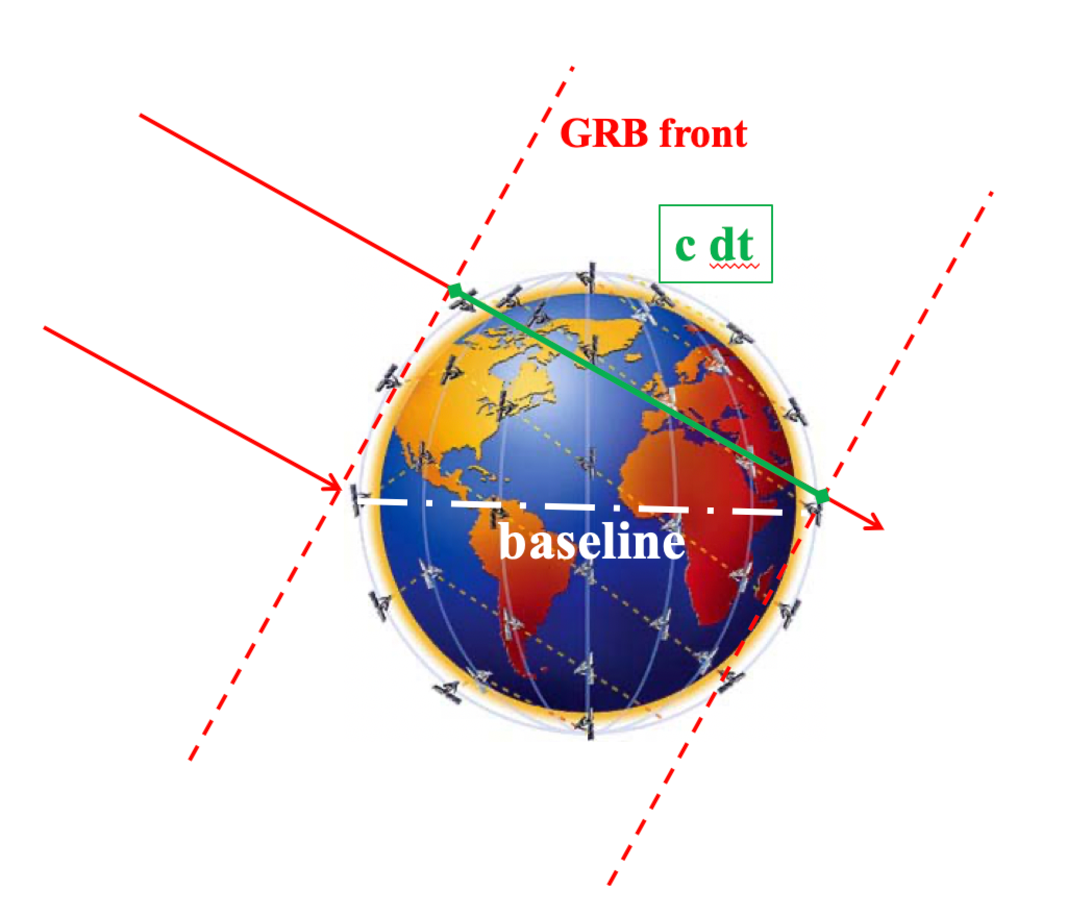
\includegraphics[height=8cm]{triangulation} 
\end{tabular}
\end{center}
\caption[example] 
%>>>> use \label inside caption to get Fig. number with \ref{}
{ \label{fig:triangulation} 
Schematic representation of the \emph{Temporal Triangulation} principle applied to a constellation of CubeSats distributed in low Earth orbits. Red arrows represent the emitted GRB photons, while the red dashed lines describe the travelling GRB front wave at different times. The green segment represents the difference in travelled distances of the GRB photons detected by two CubeSats placed at a generic baseline (white dashed line).}
\end{figure} 



\begin{comment}
\subsection{Intro Angelo}
\label{sec:intro}  % \label{} allows reference to this section


The Gamma Ray bursts are transient celestial events that are thought to be produced by the collapse of massive stars or by the coalescence of two compact objects. Their main observational characteristics are the huge luminosity and fast variability, often as short as one millisecond, with a spectral emission localized between the hard X-rays and soft Gamma rays. This phenomena have duration that can vary in each case, starting from few decimals of seconds up to hundreds of seconds. For this reason the GRBs population is catalogued according to the time scale during which the 90\% of the flux is emitted by the source (F$_{90}$). The population of Short GRBs includes bursts with T$_{90}$ $\lesssim$2 s, whilst GRBs with larger values of T$_{90}$ are catalogues as Long GRBs.
Assuming isotropic emission the energy released can attain 10$^{54}$ erg, i. e. the rest mass energy of the Sun (see e.g. Bloom et al. 2009, ApJ, 691, 723), in about 100s duration. However it is now believed that strong beaming reduces the energetic budget up to three orders of magnitude (Abdo et al. 2009, Science, 323, 1688).\\
The coalescence of compact objects, neutron stars (NS) and black holes (BH), and the sudden collapse to form a BH, are fundamental to investigate both the physics of matter under extreme conditions, and the ultimate structure of space-time. For this reason, a fast and accurate localization of the prompt emission of the GRBs is fundamental, especially for the syncronous observation of the GRB phenomenology with different observatories. 


\end{comment}

\section{Triangulation technique}
The aim of this work is to investigate the localisation capabilities of the HTP/HSP mini-constellation composed of six 3U units. The main targets that will be discussed in the following are the highly energetic high-energy transients GRBs. 

The simple and robust idea that will be applied for accurately localise the transient astrophysical sources is the so-called \emph{Temporal Triangulation}.  

To describe the principle behind the method, let us represent the transient event as a narrow wavefront (pulse) travelling in a given direction and let us displace a network of detectors in space. The narrow wavefront will hit the detectors of the network at different times that depend on the spatial position of each detector and the direction of the wavefront. As represented in Figure~\ref{fig:triangulation}, the transient event will be registered by two detectors of the network with a delay $dt$ proportional to their projected distance with respect to the source direction (green segment). The combination of the delays measured by different pairs of detectors observing the same event will allow to reconstruct its position in the sky. For the sake of description, let us consider a subset of 3 detectors distributed in the equatorial plane (panel a of Figure~\ref{fig:triangulation2}) observing simultaneously a generic event $S$ in certain position in the sky (with direction with respect to the Earth barycenter represented by the yellow dashed line). As shown in panel b of Figure~\ref{fig:triangulation2}, the delay measured $\Delta t_{BC}$ by combining the observations of the detectors B and C allows us to identify a set of infinite possible directions of the transient source belonging to a circulare base of a cone. Each of these source directions $\vec{d}_i$ satisfies the relation $\Delta t_{BC}=\vec{\rho}_{BA}\cdot \vec{d}_i$, where $\vec{\rho}_{BA}$ is the vector describing the distance between the two detectors. A similar result can be obtained by combining the measurements of the detectors B and C'. Interestingly, the superposition of these two results reduces the degeneracy in the source direction, allowing us to determine two possible positions of the source defined as the intersections of the two cones (Figure~\ref{fig:triangulation2} panel c), one of which corresponds (as expected) with the real one. Increasing the number of independent delay measurements, it is then possible to univocally localise the transient event in the sky. It is then clear that in order to achieve localisation capabilities, a generic fleet of the detectors distributed in space should guarantee the simultaneous observation of an event with at least three of its elements.    

\begin{figure}
\begin{center}
\begin{tabular}{ccc}
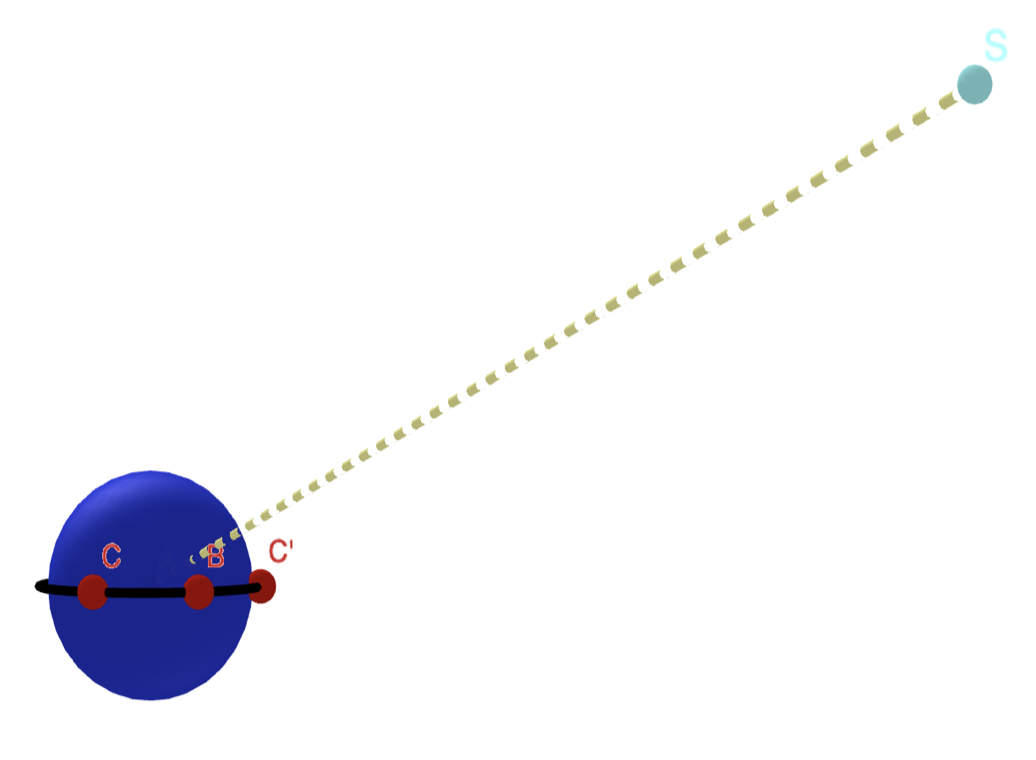
\includegraphics[height=5cm]{trinag_fig1} &
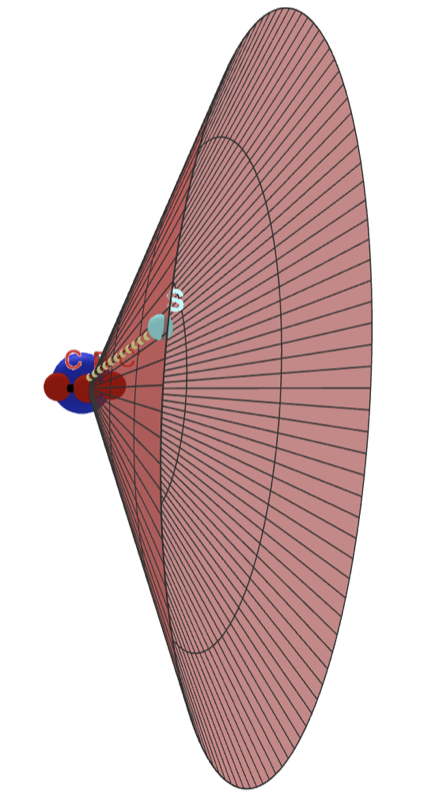
\includegraphics[height=6cm]{triang_fig2} &
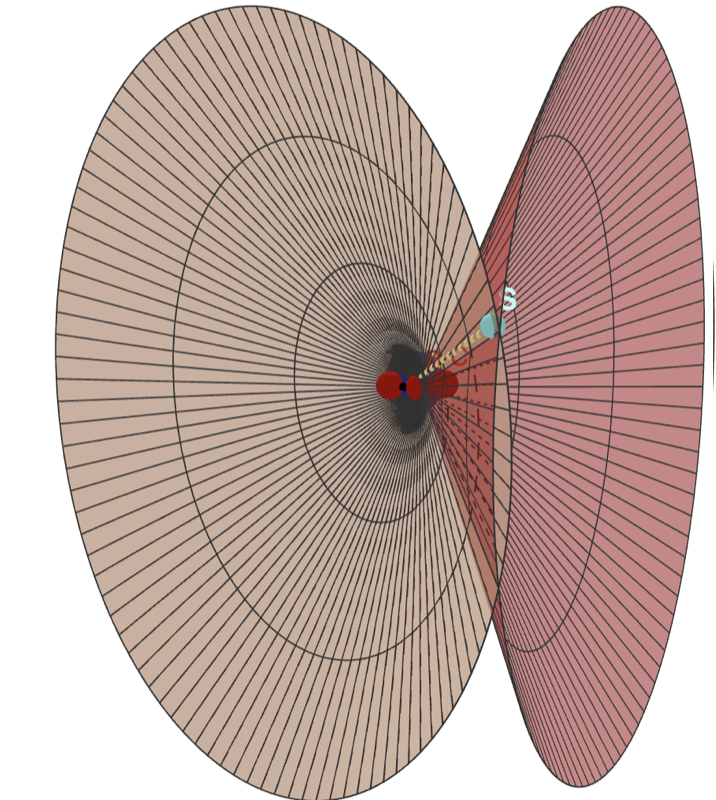
\includegraphics[height=6cm]{triang_fig3} \\
a) & b) & c)\\
\end{tabular}
\end{center}
\caption[example] 
%>>>> use \label inside caption to get Fig. number with \ref{}
{ \label{fig:triangulation2} 
\emph{Panel a)} Schematic representation of a triplet of CubeSats distributed in an equatorial plane that observed simultaneously a transient event located at the position $S$. \emph{Panel b)} Graphic representation of the infinity source directions identified using the delay measured by combining the observations of the event obtained with the detectors B and C. \emph{Panel C)} Superposition of the source directions obtained combining the delays obtained with the detector paris B-C and B-C'. The intersection of the two cones identifies two possibile locations of the event in the sky.}
\end{figure}

The description of the method reported so far does not take into account of any possible source of the uncertainty associated with the system. More in detail, the localisation capabilities of the system, hence the accuracy associated with the source position, will depend on several aspects such as the capability of reconstruct the position of the detectors during the observation of the event, the ability to recover the delay between signals observed by different detectors and the capability of the detector to precisely time tag the photons associated with the transient event. 
A first proxy on the accuracy in determining the source position $\sigma_{PA}$ can be determine in the hypothesis of an event (e.g. a GRB) whose emitted photons arrive to a series of N detectors uniformly distributed in an orbit, and it is given by the expression:

\begin{equation}
\label{eq:sigma_pos}
\sigma_{PA} = \dfrac{(\sigma_{delay}+\sigma_{tpos}+\sigma_{time})^2}{<Baseline>\sqrt{(N-1-2)}}
\end{equation}

where $\sigma_{delay}$ is the error on the delay measurement obtained combining the light-curves recorded by two detectors, $\sigma_{tpos}=\sigma_{pos}/c$ is the error induced by the uncertainties on the space localisation of the detectors, $\sigma_{time}$ is the uncertainty on the absolute time reconstruction, $<Baseline>$ is the average distance between the detectors ad N$_{ind} = N-1$ is the number of statistically independent pairs of satellites used to determine the delay measurements.\\

	
%%This relation highlights how the positional accuracy, in addition to the number of satellites making up the swarm, is strongly dependent from the uncertainty on the cross-correlation delay measurement E$_{cc}$. In order to obtain a realistic estimation of this uncertainty as a function of the GRB duration, flux and of its intrinsic variability, we have to take advantage of the current repositories of both short and long GRB data, in order to simulate as much as possible the wide phenomenological properties characterizing these transient events, as seen by the future \her mission. 


For a more accurate approach on determine the position and relative uncertainties of a generic GRB in the sky by means of time delay measurements, let us consider a swarm of $n$ satellites, each one identified by a position vector $\vec{r}_i$ (with $i=0,\dots, n-1$) with respect to a suitable reference frame, e.g. the Earth barycenter in equatorial coordinates.
To determine the GRB direction $\hat{d}$, it is possible to measure the time delays of the GRB signal as seen from each pair of  satellites. 
Defining $t_0$ the time at which the GRB signal arrives at the origin of the chosen reference frame, each $i$-th satellite will receive the GRB at a time $t_i$
\begin{equation}
  t_i = t_0 - \frac{\vec{r}_i \cdot \hat{d}}{c}.
\end{equation}
The expected time delays between two satellites will be
\begin{equation}
    \Delta t_{ij}(\hat{d}) \equiv t_j - t_i = \frac{(\vec{r}_j - \vec{r}_i) \cdot \hat{d}}{c} =  \frac{\vec{\rho}_{ij} \cdot \hat{d}}{c},
\label{eq:delayexp}
\end{equation}
where $\vec{\rho}_{ij} \equiv \vec{r}_j - \vec{r}_i$.
The real (measured) time delay between the signal recorded by two satellites $\Delta \tau_{ij}$ is inferred e.g. by applying cross-correlation techniques to the light-curves.
The direction of the GRB, e.g. its equatorial coordinates, can be estimated comparing the computed and measured delays between satellites using e.g. the non linear least squared method.
We define the $\chi^2(\hat{d})$ function as the sum the squares of the difference between the expected and observed time delay divided by its statistical error
  \begin{equation}
    \chi^2(\hat{d}) = \sum_{i = 0}^{n - 2}\sum_{j = i + 1}^{n - 1} \frac{(\Delta \tau_{ij} - \Delta t_{ij}(\hat{d}))^2}{\Theta_{ij}^2},
    \label{eq:chisq}
  \end{equation}
where $\Theta_{ij}^2$ includes the positional error on the satellites expressed in light-seconds, the accuracy in the absolute timing of the detectors, the uncertainty on constraining the time delay between the signals and any hypothetical systematic uncertainty related to the set-up or method applied.
  
The unitary vector $\hat{d}$ identifying the GRB direction can be written in terms of Right Ascension $\alpha$ and Declination $\delta$, that is
  
  \begin{equation}
    \hat{d} = \{\cos{\alpha} \cos{\delta}, \sin{\alpha} \cos{\delta}, \sin{\delta}\}.
  \end{equation}

Minimising Eq. \ref{eq:chisq} with respect to $\alpha$ and $\delta$ gives us an estimate of the direction of the GRB.
Moreover, if Eq. \ref{eq:chisq} satisfies all the hypotheses in [Y.  Anvi, 1976, ApJ, 210, 612], we can also calculate the confidence region for the GRB equatorial coordinates on the plane of the sky.






\section{EXPLOITING THE HERMES PATHFINDER LOCALISATION CAPABILITIES }

In the following, we describe in details the analysis performed, as well as the related assumptions and caveats, to investigate the capabilities of the HERMES-TP/SP mini-constellation (6 3U CubeSats) on localizing GRBs in the sky.

The key to accurately locate an event by means of the temporal triangulation method described above is to decrease as much as possible the uncertainties summarised by the term $\Theta^2$ of Eq.\ref{eq:chisq}. Starting from the HTP/SP technical properties, we can investigate the positional uncertainty budget to be able to identify the most crucial limiting factors. The final design of the spacecraft including GPS receivers and accelerometers, guarantees the possibility to reconstruct the position of the CubeSats with an accuracy smaller than 30 meters, that translates into an temporal accuracy lower than 30 ns (see SPIE PoliMi). Moreover, the absolute timing accuracy achievable from the detector is going to be lower than 0.4 $\mu$s for both the X and S modes [see SPIE Evangelista]. As we show in more detail later, considering the HERMES-TP/SP set up, we can conclude that, even for the brightest GRBs, the uncertainty on the GRB position will be dominated by the accuracy on the time delay between the GRB light-curves and possibly by unknown systematics still to be investigated. In the following we will show that on average uncertainties on the time delays obtained applying cross-correlation techniques are of the other of tenths of milliseconds, a few orders of magnitude larger than the uncertainties discussed above.

\subsection{GRB structure and time delay accuracy}

To be able to investigate the achievable accuracy in the measurement of the time delays between the arrival times for photons emitted by a generic GRB and observed by different detectors of the HTP/SP mini-constellation, we built a procedure that includes the creation of GRB templates, the application of cross-correlation techniques as well as Monte Carlo simulations.

As a first step, we searched the available Fermi GBM archive seeking for GRBs characterised by variability on time scales as short as a few milliseconds. The hypothesis being that fast variability should enhance the sensitivity on time delay measurements, especially when the statistics of the available data is relatively limited. We then isolated two candidates, one belonging the so-called short GRBs and the other from the long class. More specifically, the short GRB (id. GRB120323507) has been observed on 2012 March 23, and it is characterised by a $t_{90}$\footnote{Time interval in which the integrated photon counts increase from 5\% to 95\% of the total counts.} duration of $\sim0.4$ seconds with a fluence of $\sim1\times10^{-5}$ erg cm$^{-2}$. On the other hand, the long GRB (id. GRB13052327) has been detected on 2013 May 2, and it is characterised by a $t_{90}$ duration of $\sim24$ seconds with a fluence of $\sim1\times10^{-2}$ erg cm$^{-2}$.

The data collected from the GBM catalogue includes light-curves from the sodium iodide (NaI) scintillators and from the cylindrical bismuth germanate (BGO) scintillators, both having a collecting area of about 125 cm$^2$. The NaI detectors are sensitive to energies included between few keV up to about 1 MeV, while the BGO detectors cover the energy range 150 keV to 30 MeV. We selected data captured with the so called \textit{Time-tagged event (TTE)} format, where the GRBs are continuously recorded with a time resolution of 2\us, within an time interval that includes 15-30 s of pre-trigger information and about 300 s of data after the trigger time.

To be able to recreate the GRB light-curves as seen by the HTP/SP detectors, we selected the energy range 50-300 keV at which corresponds to the largest effective area of scintillators (around 50 cm$^2$). For this reason, data collected from the GBM observations has been previously filtered in order to have events only in this energy range.

The need to generate GRB templates (functional forms of the GRB light-curves) comes from two crucial aspects in the procedure follow to investigate the measurement of signal delays: a) flexibility to recreate GRB light-curves independently of the detectors effective area and b) the possibility to simulate GRB light-curves with intrinsically poor statistics.  

Indeed, simulations on short time scales ($\sim$1 ms) of a unique-like type of transient events such as a GRB, based on observed light-curves, can be challenging when the effective area of the detector is so small that the statistic is fully dominated by Poissonian fluctuations that unavoidably characterised the (quantum) detection process. In particular, if the detected counts within the given time scale is $\leq1$, quantum fluctuations of the order of 100\% are expected. If, naively, the number of counts per bin is simply rescaled to account for an increase effective area, these quantum fluctuations can introduce a false imprint of 100\% variability with respect to the original signal. No definite cure is available to mitigate this problem, that could be, however, alleviated by rebinning and/or smoothing techniques. Although smoothing techniques allows the creation of light curves for a desired temporal resolution, correlation between subsequent bins is unavoidable. Cross-correlation techniques are strongly biased by this effect, therefore we opted for a more conservative method implying standard rebinning in which the number of photons accumulated in each (variable) bin is fixed. After several trials and Monte-Carlo simulations, we found that 6 photons per bin allows to preserve the signal variability introducing undesired fluctuations not larger than $\sim$30\%. Applying this rebinning techniques to the GBM light-curves (at the maximum time resolution of 2\us), we generated a variable bin size light-curves. In order to generate a template usable on any time scale, we linearly interpolated the previous light-curve to create a functional expression (template) for the theoretical light-curves. We note explicitly, that linear interpolation between subsequent bins is the most conservative approach that does not introduce spurious variability on any time scales. For a given temporal bin size, it is then possible to rescale the GRB template previously described in order to match the requested effective area (e.g. that of the HTP/HSP detectors), generating then the expected number of photons within the time bins. In addition, before and after the burst, we rescaled the background on the GRB template to match the nominal background collected the detector as predicted with respect to the CubeSat orbits. Figure~\ref{fig:template_short_long} shows the templates (red lines) for the long (left panel) and short (right) GRBs generated by following the procedure described above. 


\begin{figure*}[h!]
\centering
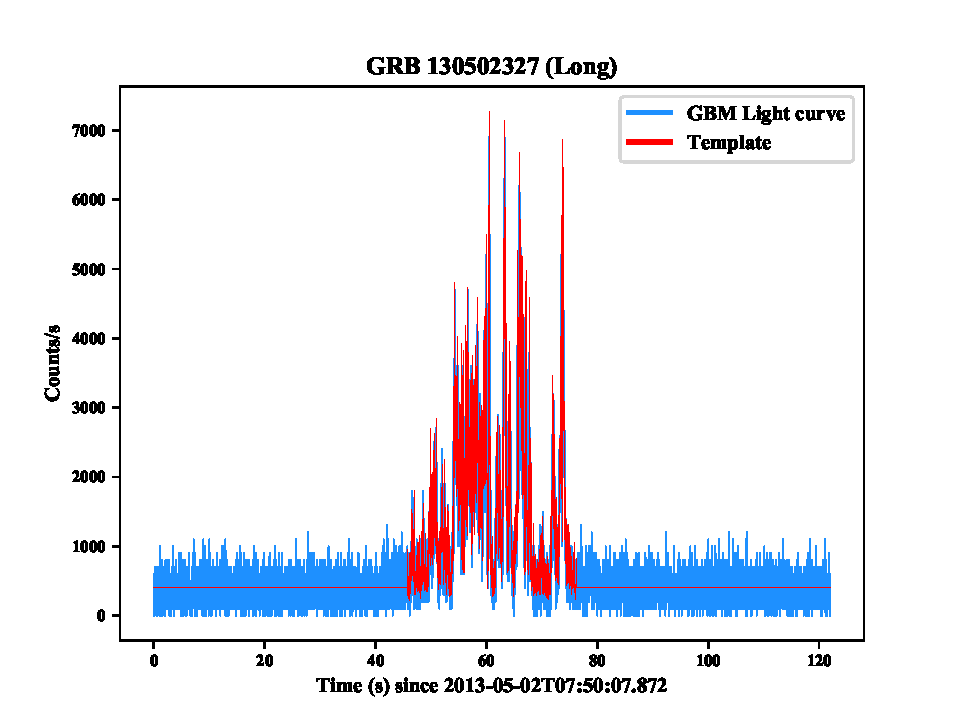
\includegraphics[scale=0.52,angle=0]{fig/Template_comparison_Long.pdf}
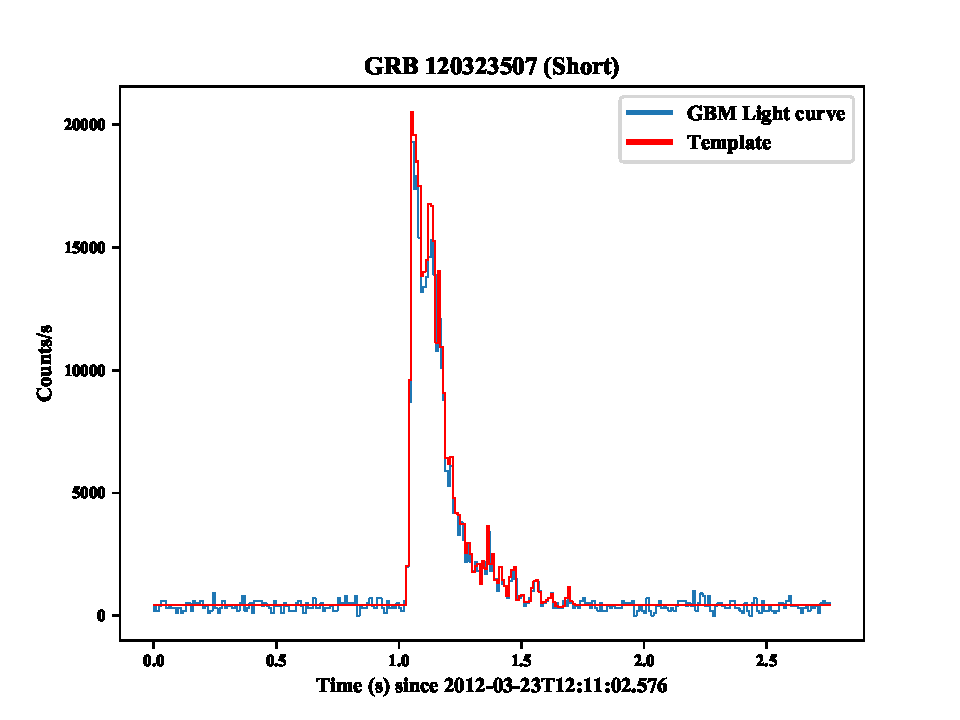
\includegraphics[scale=0.52,angle=0]{fig/Template_comparison_Short.pdf}

\caption{The Fermi/GBM light curves of the long GRB 130502327 (left panel) and of the short GRB 120323507 (right panel) and the relative \textit{template} (red line) obtained with the procedure described in the text. In both cases, for reasons of clarity, we used a bin time of 10$^{-2}$ s for the light curves and templates of both the GRBs.} 
\label{fig:template_short_long}
\end{figure*}

Starting from the GRB templates we generated light-curves by rescaling the detector effective area to match that of the HTP/HSP mini-constellation and by applying a Poissonian randomization of the counts contained in each bin of the template. We then applied standard cross-correlation techniques (\textbf{ref}) using two light-curves with the aim to determine the time delay between two signals. Since we are interested in reconstructing the accuracy achievable in the time delay, and not stringily on the delay per se, we did not shift in time the template to simulate the signals. To extract the temporal information of the delay, we fitted a restricted region around the peak of the cross-correlation function with an \emph{ad hoc} model composed of an asymmetric double exponential component. The uncertainty associated with the location (in delay) of peak of the cross-correlation function defines the accuracy on determine the delay between the two detected signals. In Figure~\ref{fig:xc_profiles} we report the cross-correlation functions obtained by cross-correlating the simulated light-curves of the long GRB 130502327 (left panel) and the short GRB 120323507 (right panel) as seen by the HTP/HSP detectors assuming an on-axis detection. Moreover, in the insets of Figure~\autoref{fig:xc_profiles} we report the zoom of the peak of the cross-correlation functions and the relative best-fitting model (red solid line).
	


\begin{figure}[h!]
\centering
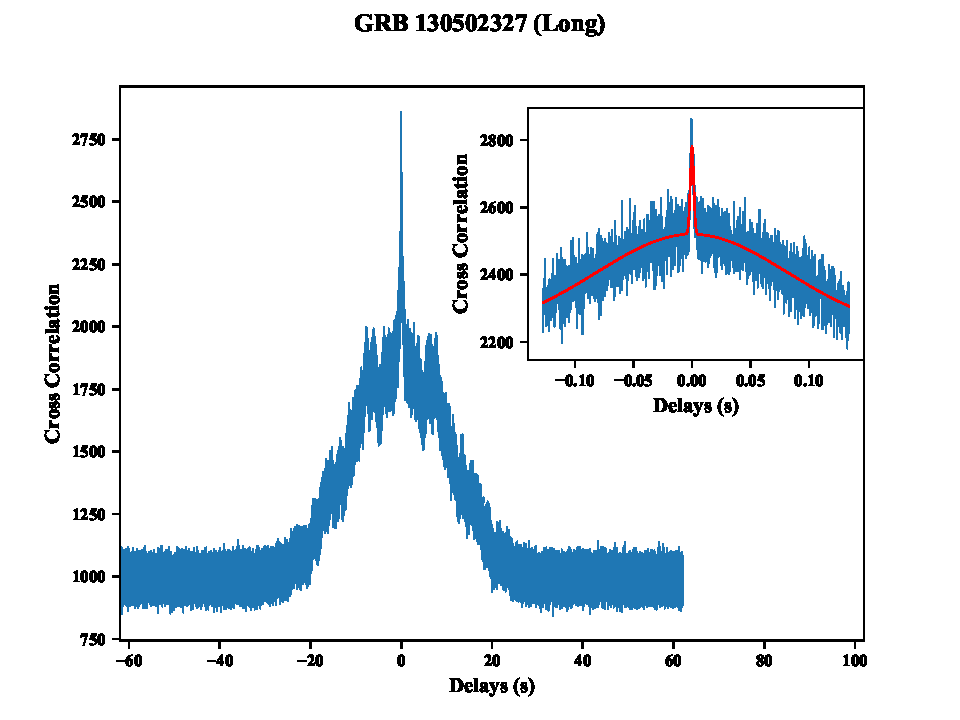
\includegraphics[scale=0.52,angle=0]{fig/CrossCorrelation_fit_LONG.pdf}
\includegraphics[scale=0.52,angle=0]{fig/CrossCorrelation_fit_Short.pdf}

\caption{Cross-correlation functions obtained by simulating the GRB light-curves of the long GRB 130502327 (left panel) and of the short GRB 120323507 (right panel) using the templates shown in \autoref{fig:template_short_long} rescaled to match the effective area of the HTP/HSP detectors. The insets report a zoom-in of the cross-correlation profiles around the peak as well as their best-fitting model (red solid line).} 
\label{fig:xc_profiles}
\end{figure}

\emph{How reliable is the fitting of the cross-correlation peak in terms of determining the accuracy of time delays between the two light-curves?} Given the complexity of an analytic approach to the problem, we decided to tackle the issue taking advantage of Monte Carlo simulations. More precisely, for each GRB, we generated 2000 light-curves by means of Poissonian randomisation of the template are we generated 1000 cross-correlation functions. For each cross-correlation function, we then determined the delay between the light-curves by fitting the peak of the function as described above. From the overall distributions of delays obtained for the long and short GRBs(left and right panels in \ref{fig:xc_sigma}) we estimated the standard deviations $\sigma_{cc-short}\sim1.2\times10^{-3}$s and $\sigma_{cc-long}\sim 8.2\times10^{-5}$s, respectively, that we interpret as a realistic estimate of the accuracy on the time delay measured with this procedure. It is worth noting that for the long GRB the mean uncertainty (obtained by averaging the results from the 1000 simulations) on the time delay obtained by fitting the peak of the cross-correlation function is only 20\% larger than with respect to  the sigma of the time delay distribution. On the other hand, for the short GRB the uncertainty on cross-correlation peak is almost a factor of 4 smaller with respect to the sigma of the peak distribution \textbf{da verificare}.


\begin{figure}[h!]
\centering
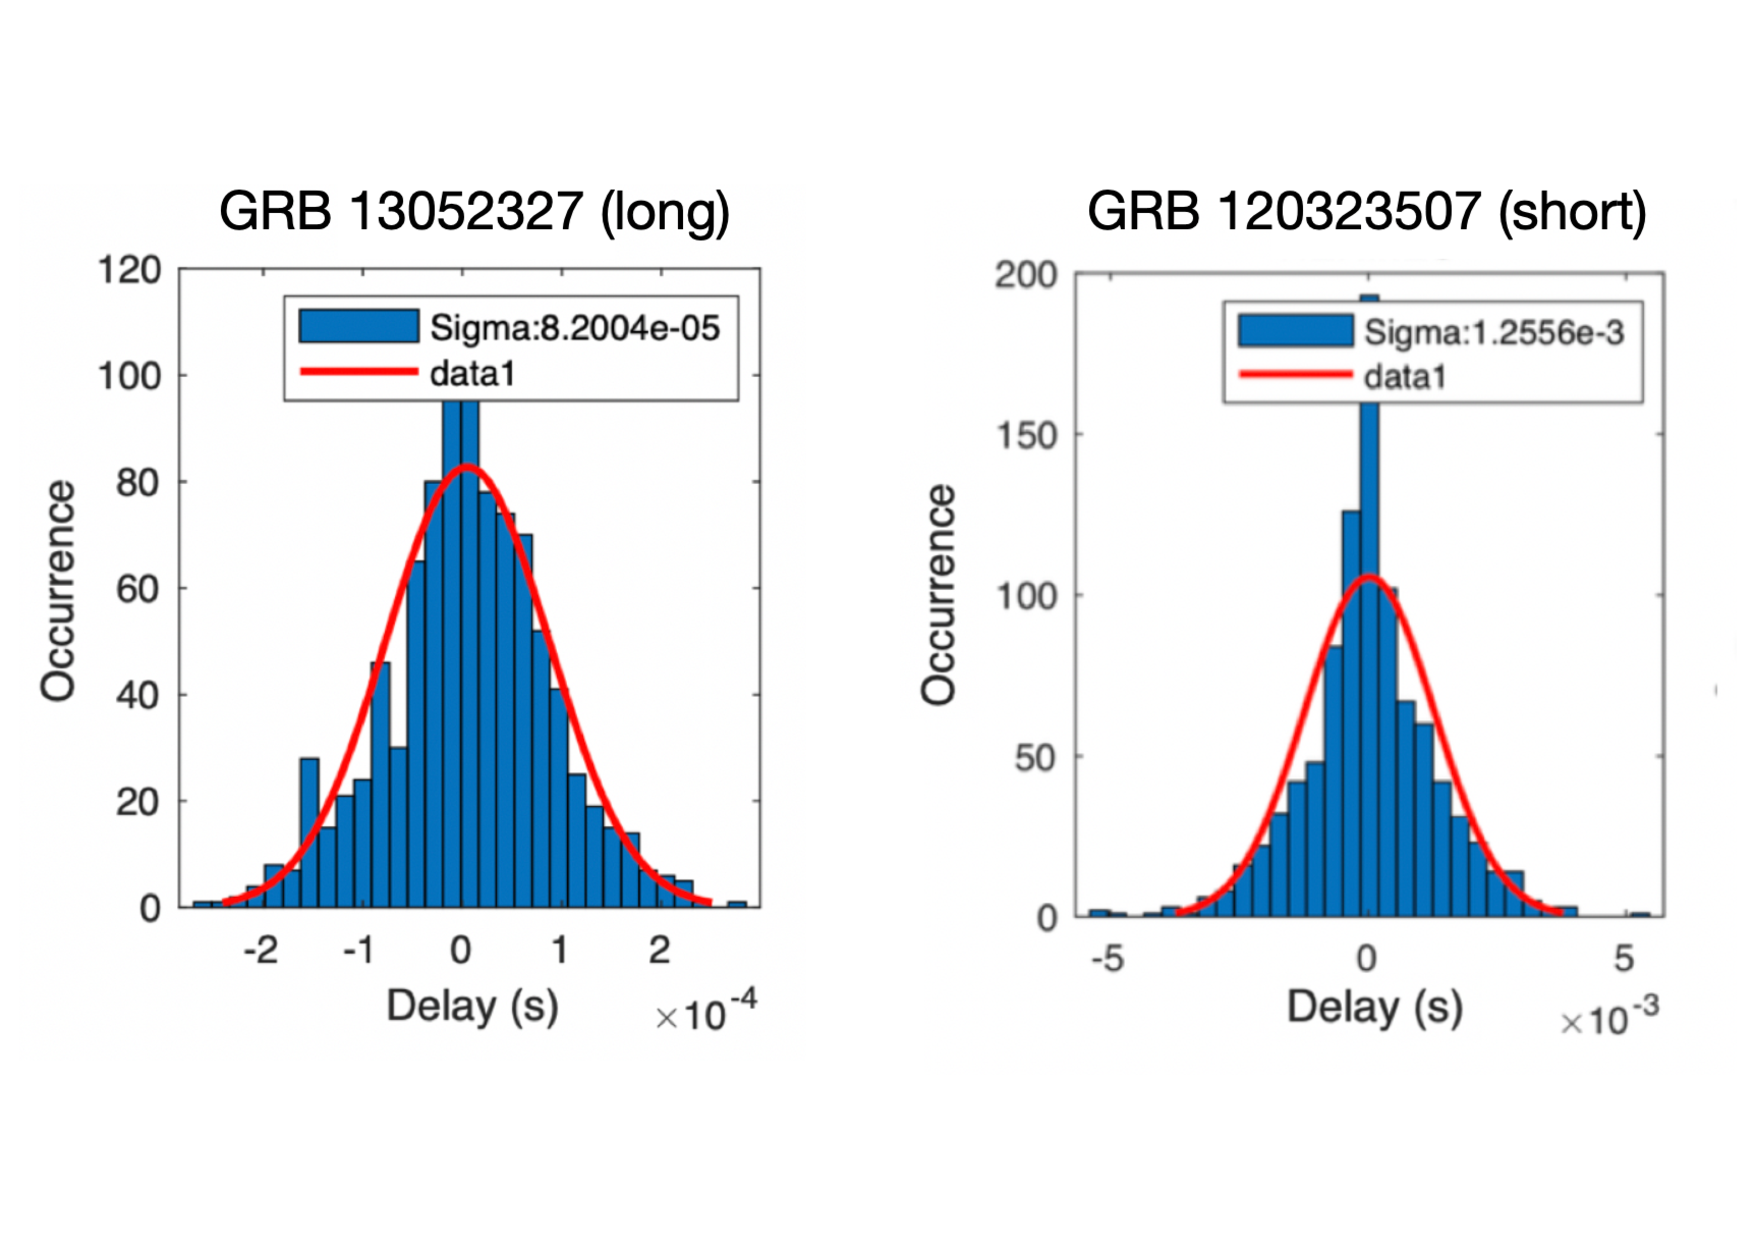
\includegraphics[scale=0.45,angle=0]{sigma_cc_sim}
\vspace{-1cm}
\caption{Distribution of delays obtained applying cross-correlation techniques to pairs of simulated light curves of the long (left panel) and short (right panel) GRBs rescaled to match the HTP/HSP effective area. The distributions are the result of 1000 Monte-Carlo simulations (see text for more details). The overlaid red line represents the best-fit normal distribution to the data.} 
\label{fig:xc_sigma}
\end{figure}

\emph{How does the GRB morphology affect the capability to accurately determine time delays by cross-correlation techniques?}
As a first attempt to test the dependence of the cross-correlation uncertainty on the brightness and temporal structure of the GRBs, we applied the technique described above to two unbiased random samples each including 100 short and 100 long GRBs selected from the available Fermi GBM catalogue.
The randomness of the samples guarantees a good coverage of the vast variety of phenomenologies, fluxes, durations and intrinsic variability that were recorded during the Fermi mission up to the moment in which this paper was written. For the long GRBs, the sample includes bursts having net fluxes ranging between 0.16 and 26 ph cm$^{-2}$ s$^{-1}$, durations between 3 and 138 s, and fluence values between 1.67 and 4 ph cm$^{-2}$. On the other hands, the sample of short GRBs ranges in flux between 0.6 and 188 ph cm$^{-2}$ s$^{-1}$, durations between 0.03 and 1.9 s and fluence values between 0.2 and 75 ph cm$^{-2}$.\\

For each burst, we simulated 2000 light-curves that allowed us to generate 1000 cross-correlation functions. Following the procedure described above, we then determined the time delay by fitting the interval near the peak with an \emph{ad hoc} (e.g. Gaussian functions, combination of two Gaussian profiles having a common centroid and asymmetric double exponential functions). The top left (top right) panel in Figure~\ref{fig:sigma_sample} shows the distributions of the time delay uncertainties (each representing the standard deviation of 1000 Monte-Carlo simulations) estimated cross-correlating the sample of long (short) GRBs. We note that an accuracy equal or smaller than 1ms is obtained for 55\% of the long GRBs (Figure~\ref{fig:sigma_sample} top-left panel, red area), while an uncertainty equal or smaller than 5ms is obtained for 30\% of the short GRBs (Figure~\ref{fig:sigma_sample} top-right panel, red area). Finally, it should be emphasized that systematic cross-correlation simulations play a crucial role in terms of investigating systematic uncertainties on the method to localize the GRBs. The bottom left and right panels of Figure~\ref{fig:sigma_sample} represent the dependence of the cross-correlation accuracy as a function of the GRB flux for the long and short GRB, respectively. As expected, stronger GRBs allow to recover time delays with a better accuracy.    


\begin{figure}
\begin{center}
\begin{tabular}{cc}
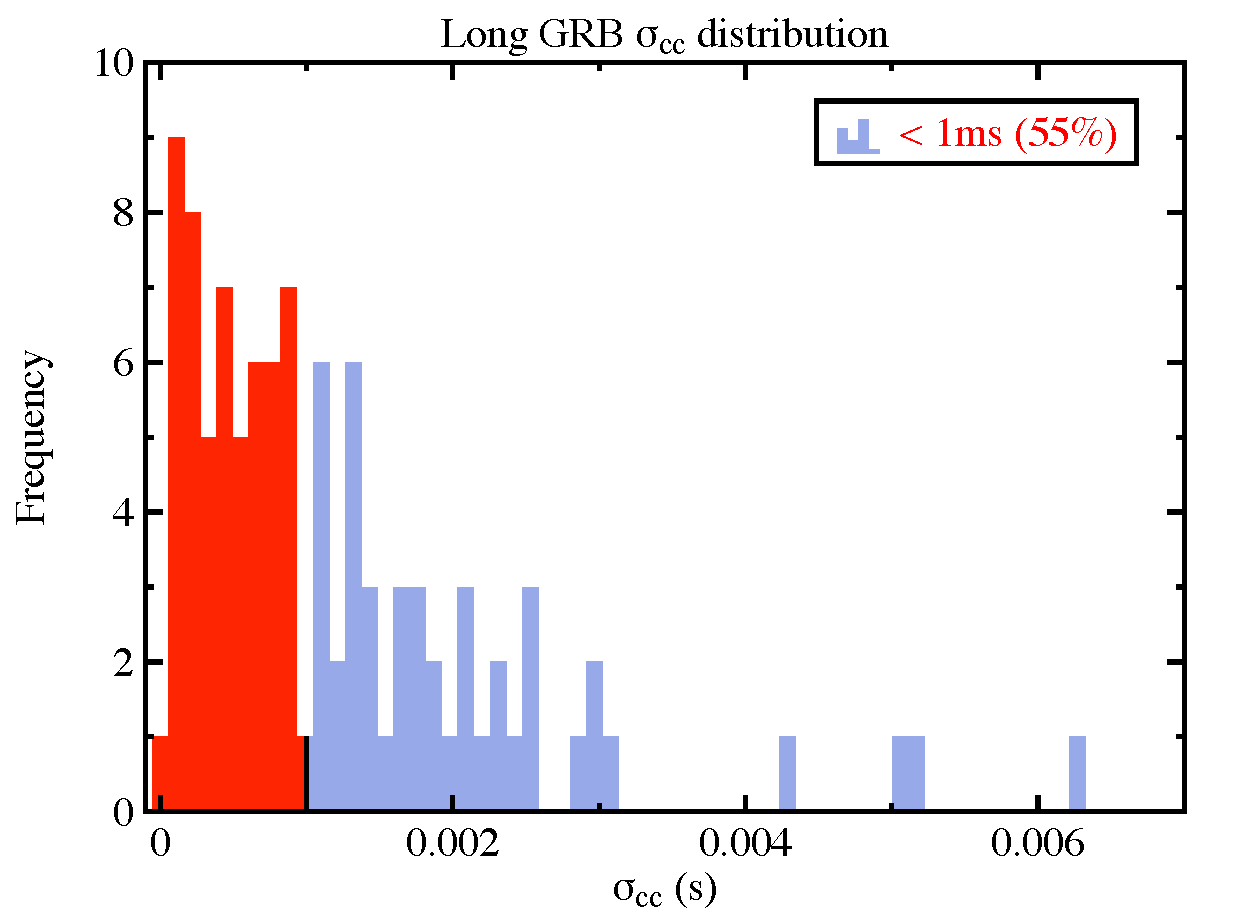
\includegraphics[height=6cm]{Long_GRB_sigma_dist} &
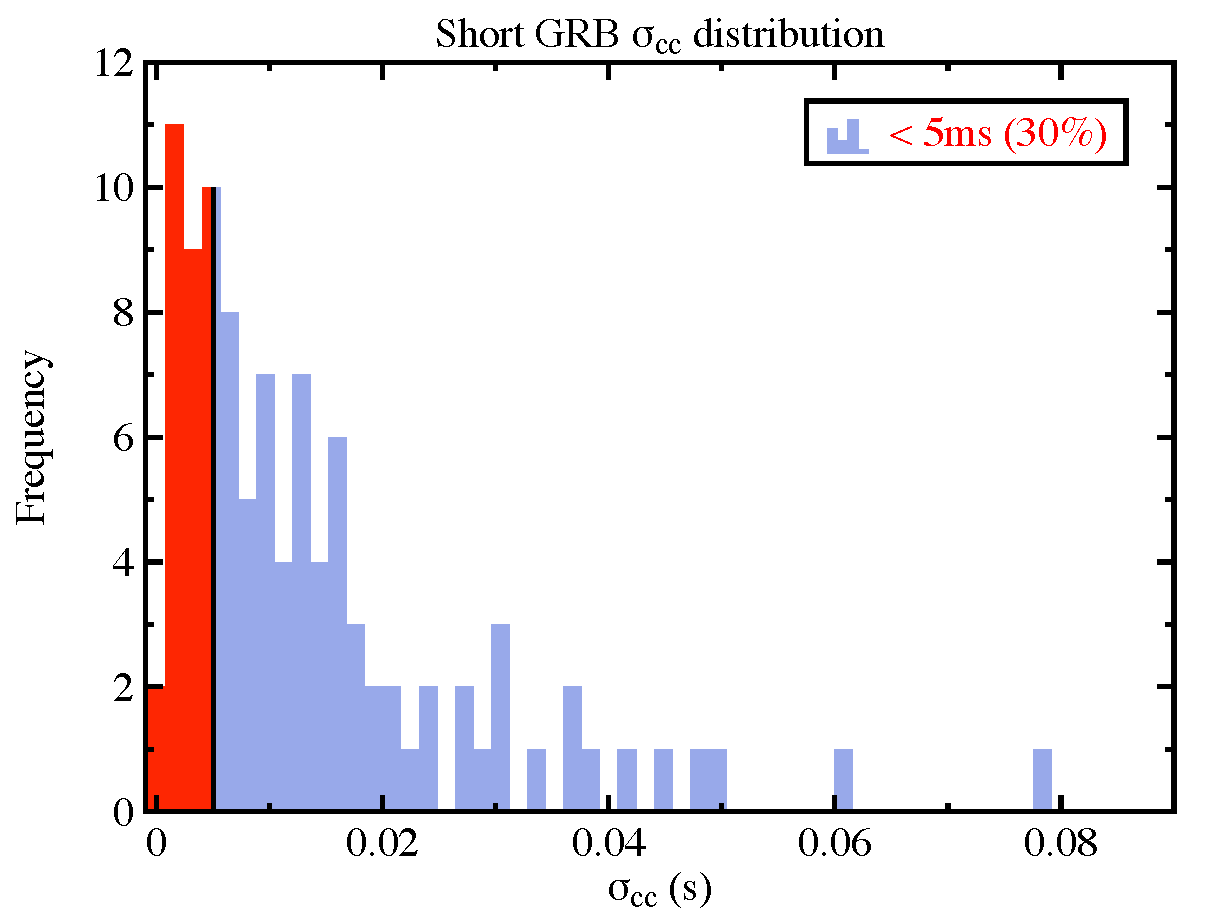
\includegraphics[height=6cm]{short_GRB_sigma_dist} \\
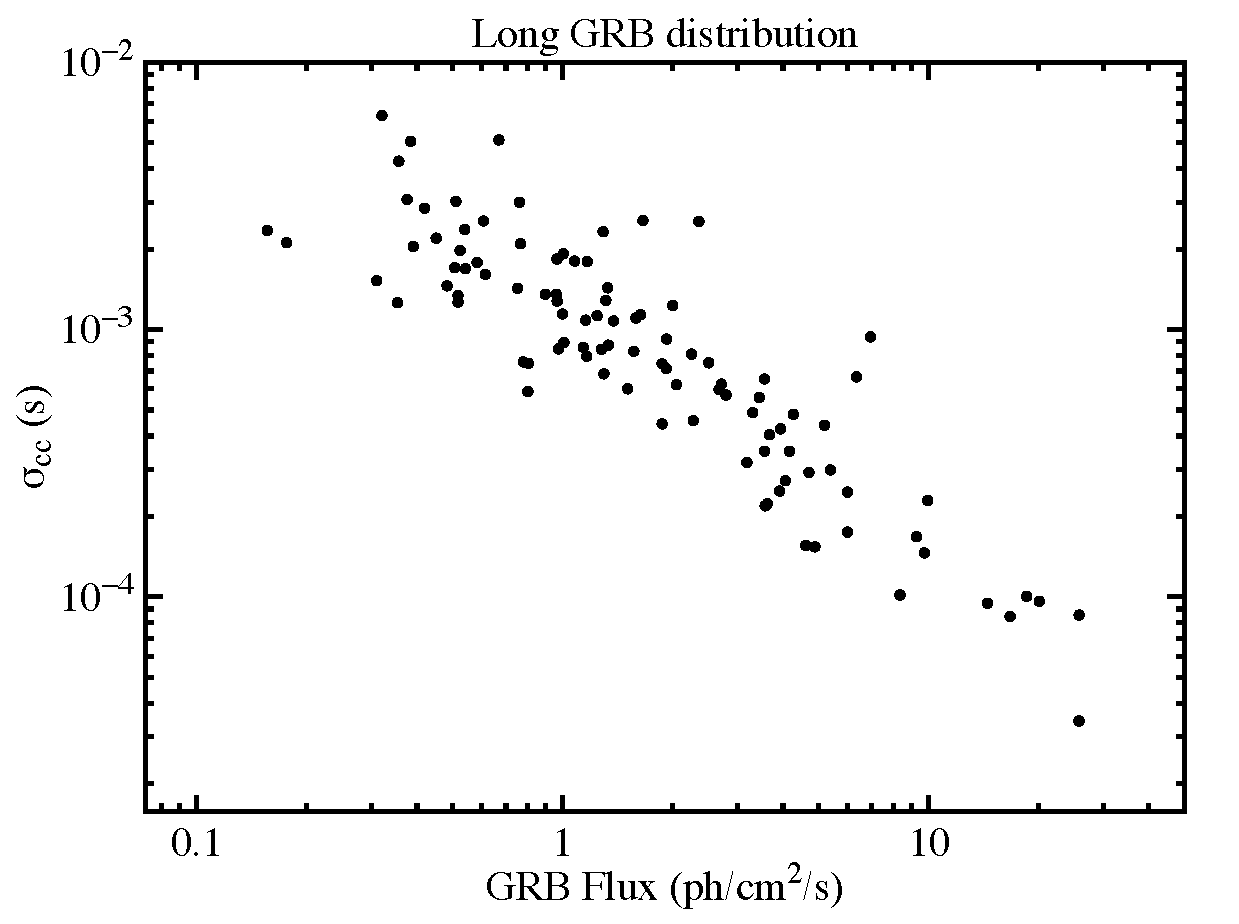
\includegraphics[height=6cm]{Long_GRB_sigma_flux} &
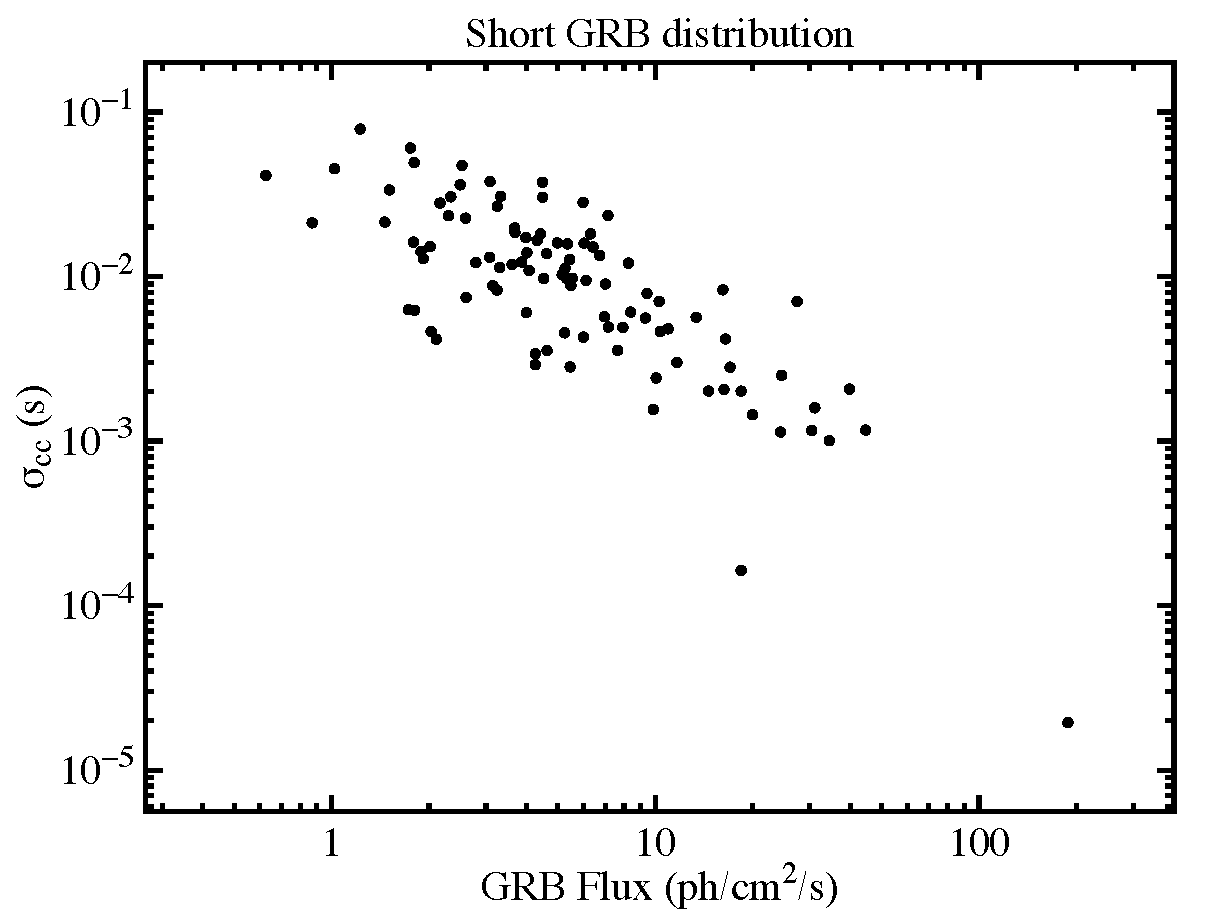
\includegraphics[height=6cm]{short_GRB_sigma_flux} \\
\end{tabular}
\end{center}
\caption[example] 
%>>>> use \label inside caption to get Fig. number with \ref{}
{ \label{fig:sigma_sample} 
\emph{Top Left panel:} distribution of the delay accuracy estimated via cross-correlation techniques a random sample of 100 long GRB selected from the Fermi GBM catalogue. In red we highlighted the sub-sample (50\%)characterised by $\sigma_{cc} < 1$ ms. \emph{Top Right panel:} distribution of the delay accuracy estimated via cross-correlation techniques a random sample of 100 short GRB selected from the Fermi GBM catalogue. In red we highlighted the sub-sample (30\%) characterised by $\sigma_{cc} < 5$ ms. \emph{Bottom Left panel:} cross-correlation accuracy as a function of the GRB flux for the sample of long GRB. \emph{Bottom Right panel:} cross-correlation accuracy as a function of the GRB flux for the sample of short GRB.}
\end{figure}


\subsection{mission scenario}
Testing the localisation capabilities of the HTP/HSP mini-constellation requires the definition of a specific mission scenario. In the following, we will give a brief description of the experimental set up used to the analysis described in this work, that is the outcome of a long mission analysis investigation performed during the first year of the project.

\subsubsection{Low Earth Equatorial Orbit}
To achieve to scientific goals of the mission, the HTP/HSP orbit has been accurately investigated and finally restricted to a low Earth orbit with altitude between 500 and 600km and inclination <20deg. Within the specific framework of the analysis reported here, the adopted reference orbit have the following properties:

\begin{itemize}
\item altitude h=550 km;
\item circular orbit (eccentricity = 0);
\item Equatorial orbit (inclination = 0).
\end{itemize}


\subsubsection{Space segment injection strategy}
The space segments injection strategies explored in mission analysis are the following:
\begin{itemize}
\item Dedicated multiple injections - one per satellite - into different true anomalies at $t_0$; 
\item Single injection of each triplet with imposed relative motion among the spacecraft belonging to the same triplet, imposed by the deployer release spring.
\end{itemize} 

As resulted from the analysis, the first option is highly sensitive to the release conditions, e.g. natural perturbations provoke a relative drift which is emphasized by the launcher and deployer injection uncertainties jeopardizing this strategy robustness in terms of scientific outcome. This option requires a dedicated launch for the HERMES Pathfinder mission. 
On the other hand, the second option is feasible without a dedicated launch, since the triplet elements can be released in a single launch event with no dedicated injection manoeuvre. The relative motion between the satellites is actually imposed by the deployer spring authority which overcomes the natural perturbations effects and the launcher injection uncertainties, making more reliable the expected scientific outcomes foreseen in the design phase. 
Here, we will consider the second injection strategy to perform the localization test.

\begin{figure}[h!]
\centering
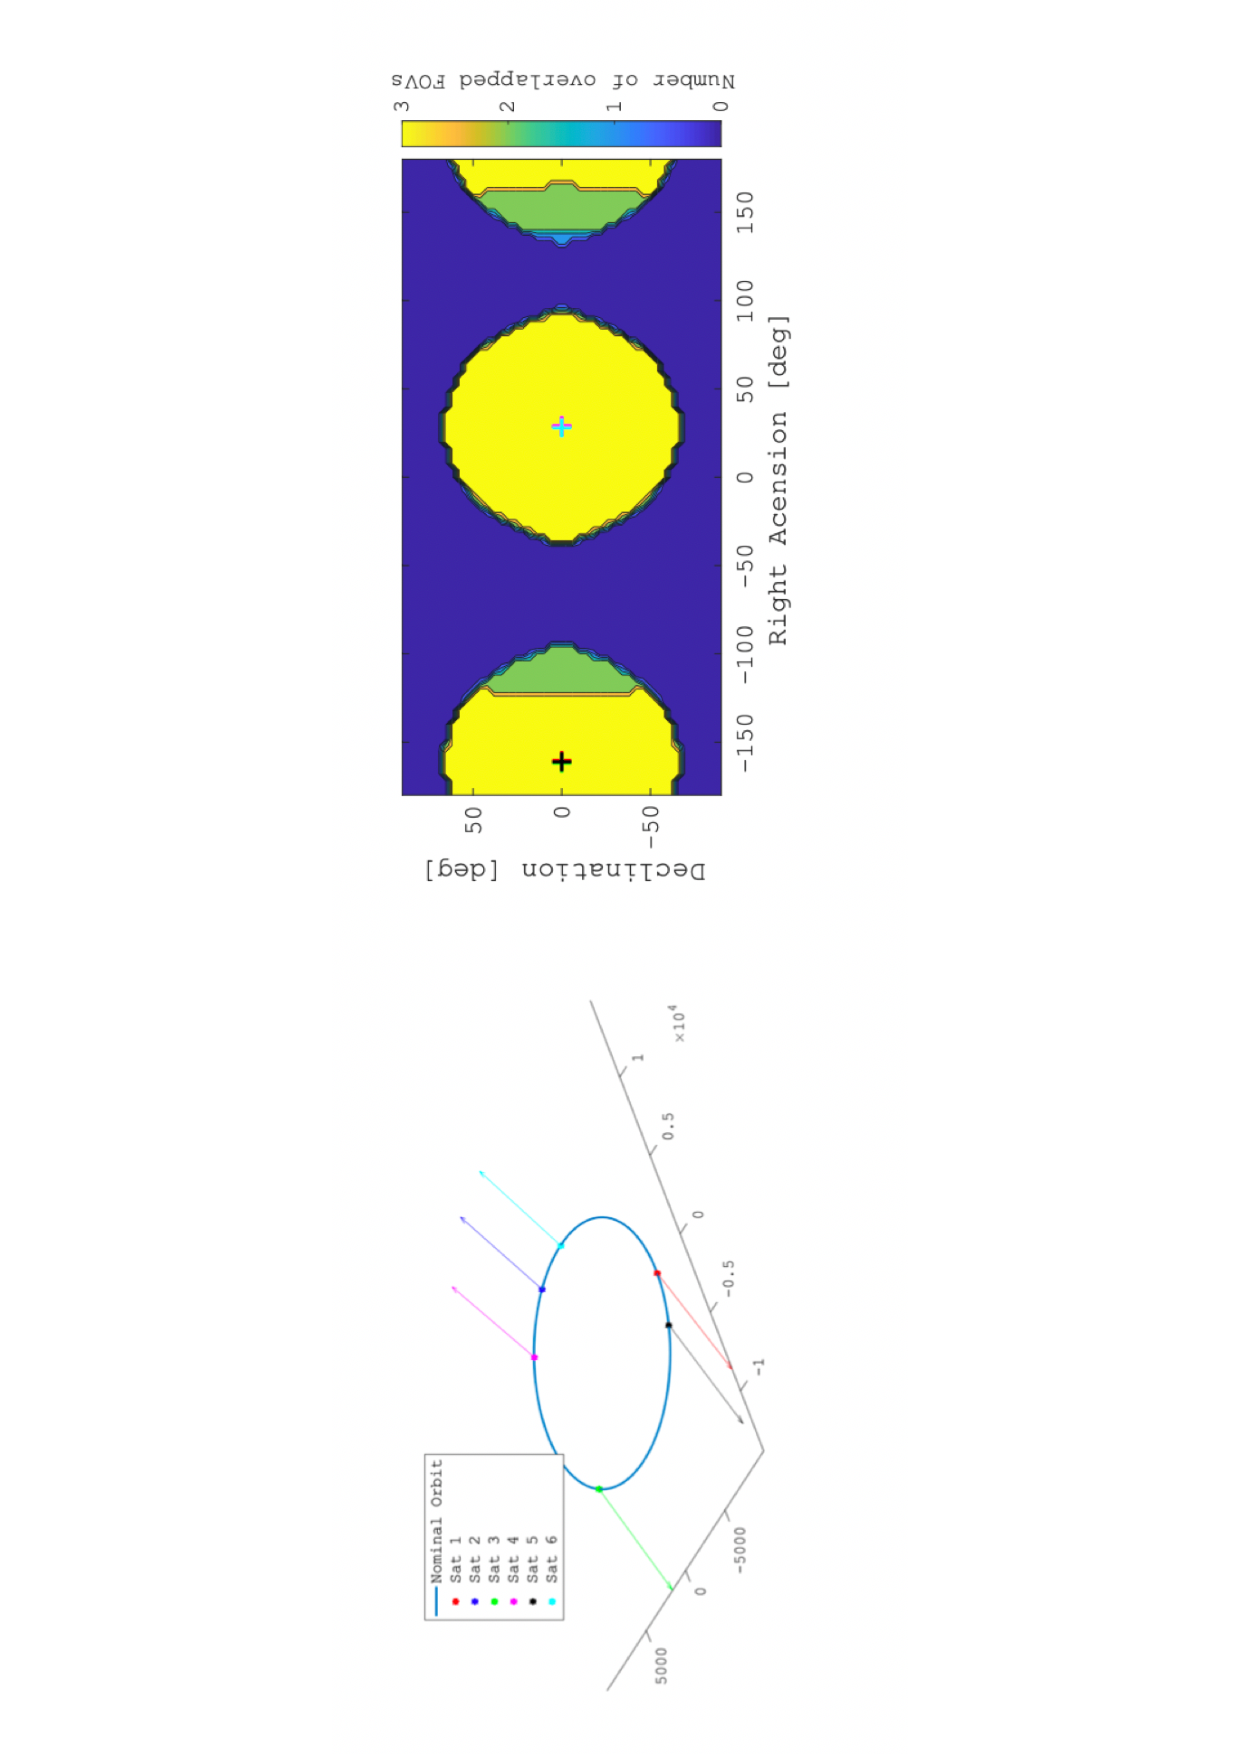
\includegraphics[scale=0.45,angle=-90]{pointying_strategy}
\vspace{-2.5cm}
\caption{LVLH optimal pointing strategy} 
\label{fig:strategy}
\end{figure}

\subsubsection{Pointing strategy}
The selection of the nominal pointing strategy significantly affects the HTP/HSP performances in terms of detection and localization of GRBs. During the mission analysis and the spacecraft design activity, specific trade-off studies have been carried out on the topic taking advantage of the quite advance attitude control performances of the HERMES CubeSats. In fact, the pointing direction of the payload’s Line Of Sight (LOS) can be controlled and even varied along the mission time-line, according to the short-medium planning for the payload utilization, compliant with the space segment capabilities, to maximize the science mission outcome. 
Three different pointing strategies have been explored:
\begin{itemize} 
\item Zenith pointing for each payload LOS; 
\item Co-alignment of $n\geq3$ payload LOSs on an Inertial-selected direction; 
\item Co-alignment of $n\geq3$ payload LOSs on a LVLH-selected direction (i.e. LOSs aligned on the zenith direction of a specific satellite in the fleet).
\end{itemize} 

The third pointing strategy, that will be used for the analysis discussed in this document, is preferred to maximize the scientific outcome of the mission. To do that, periodical optimization of the LOS direction of each satellite are foreseen in order to maximize the overlapping Field of View (FoV) and hence the number of GRBs potentially triangulated. More in details, the whole mission is divided in periods (from days to weeks) in which the pointing directions of each satellite is kept fixed in the non-inertial LVLH (Local Vertical-Local Horizontal) reference frame. The pointing direction of each satellite in the LVLH frame is uniquely defined by two angles: the first, in the orbital plane, is the angular displacement between the LOS and the radial direction, and the second is the elevation of the LOS above (or below) the orbital plane. During each period, the optimal set of angles (two for each satellites) is selected using a heuristic particle-swarm optimization algorithm to maximize the scientific return, i.e. the number of GRBs triangulated during that frame time. Figure~\ref{fig:strategy} shows the position and pointing of the HTP/HSP detectors within the LVLH pointing strategy (left panel) as well as the associated map of the overlapping FoVs.  



\subsubsection{Simulation strategy}
To investigate the level of accuracy on the detection and localization of GRBs with respect to the mission scenarios previously described we adopted the following strategy: 
\begin{itemize}
	
\item following the results reported in the Fourth Fermi-GBM GRB catalogue [\citenum{vonKienlin20}], we generated GRB events assuming a uniform distribution in the plane-of-the-sky. The number of simulated GRBs during the mission duration (2 years) reflects the Fermi GBM detection rate $\alpha_{GBM} \simeq 0.083$ GRB/sr/d, which corresponds approximately to a total of 760 GRB events in the whole sky ($4\pi$ steradians) within the assumed HTP/HSP mission life-time; 

\item we temporally located the 760 simulated GRB events by sampling uniformly at random from the time data-set associated to the positions of the fleet elements. More specifically, we randomly extracted 760 time-intervals (1-minute length) among the 1051201 available from the simulation of the satellite positions. With that, we are assuming that the process of detection of a GRB has a duration shorter or equal to 1 minute. We note that this assumption is surely valid for short GRBs, whilst it is not applicable for 30\%-40\% of the long GRBs showing duration larger than 60 seconds; 

\item for each GRB event, we determined the number of active satellites (non-transiting within the South Atlantic Anomaly) able to detect it, by verifying that the direction of the GRB and the LoS of the instrument identify an angle lower or equal 60 degrees. This guarantees that the GRB event falls within the $3\pi$ steradians FoV (Full Width at Half Maximum) of the detector. 

\item we processed only GRB events observed by a minimum of 3 satellites, or equivalently, for which a minimum of 3 satellites have the GRB in their FoVs. This guarantees the possibility to apply \emph{Temporal Triangulation} techniques to determine the position of the GRB in the sky. 

\end{itemize}

For each of the GRB potentially localizable, we determined the expected time delays $\Delta t_{ij}(\hat{d})$ between pairs of satellites by using Eq.~\ref{eq:delayexp}. The associated real (measured) time delay $\Delta \tau_{ij}$ will be then generated as:
\begin{equation} 
     \Delta \tau_{ij}=\Delta t_{ij}(\hat{d})+N(0,\sigma_{cc}),
\end{equation}              
where $N(0,\sigma_{cc})$ is the cross-correlation uncertainty randomly extracted assuming a normal distribution with zero mean and standard deviation equal to the results obtained from the analysis of the sample of long and short GRBs described above. More specifically, among the 760 GRBs, 83\% (following to Fermi GBM statistics) will be simulated assigning characteristics of the long GRBs and $\sigma_{cc-long} = 1$ ms, while the remaining 17\% will be simulated as short GRBs with $\sigma_{cc-short} = 5$ ms.
Using Eq.~\ref{eq:chisq}, we then calculated a $\chi^2$ map of the whole sky by creating a grid of points uniformly sampling the equatorial coordinates. Finally, we estimated the most probable position of the simulated GRB by calculating the values of $\alpha$ and $\delta$ that minimise the $\chi^2$ function. Confidence intervals at $1\sigma$ level represent the coordinate intervals $\sigma_\alpha$ and $\sigma_delta$ for which $\Delta \chi^2 (\hat{d}) = 
\Delta 
\chi^2(\nu, 68\%)$, where $\nu$ is the number of parameters in the function. We emphasise that the coordinate intervals obtained by marginalising the confidence region, especially $\sigma_\alpha$, can be overestimated. 


\begin{figure}
\begin{center}
\begin{tabular}{cc}
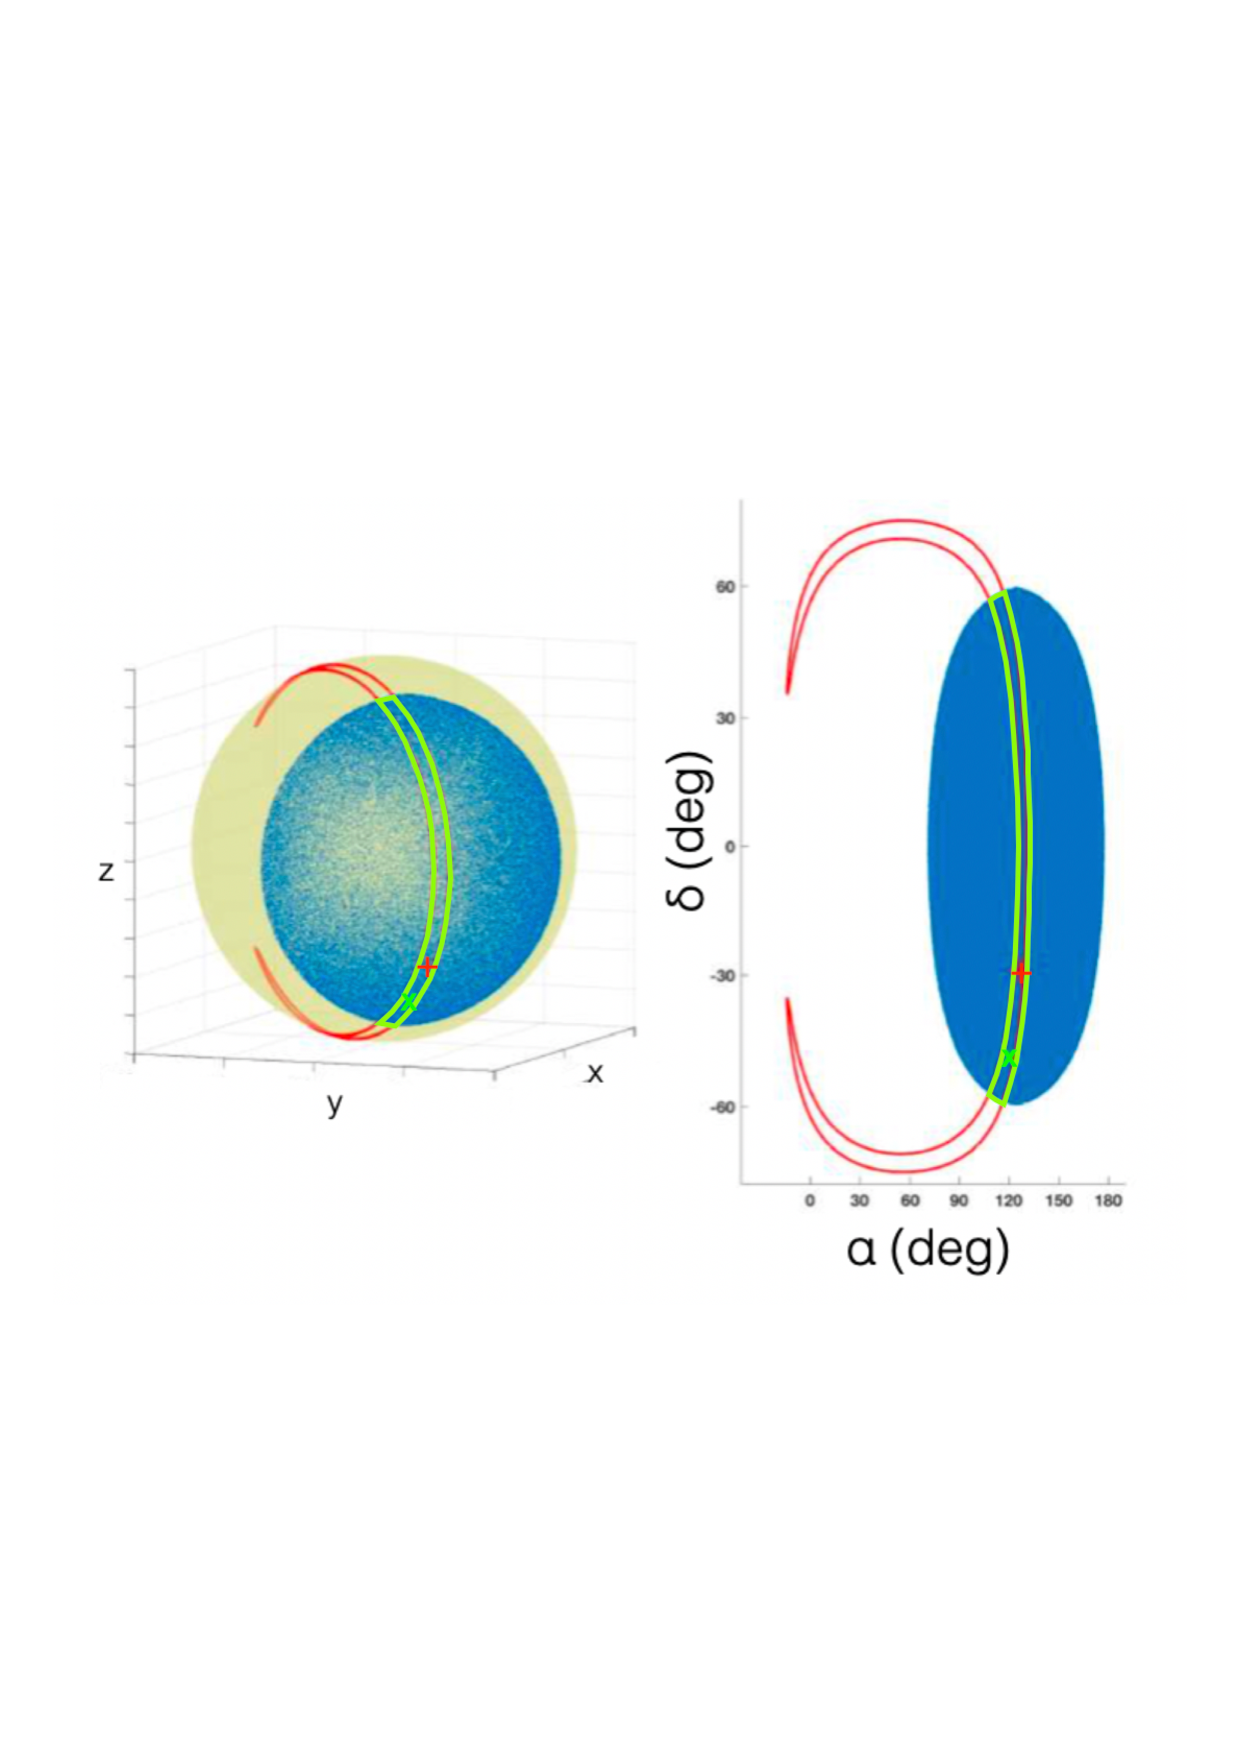
\includegraphics[scale=0.4,angle=0.0]{fig_loc_30deg} &
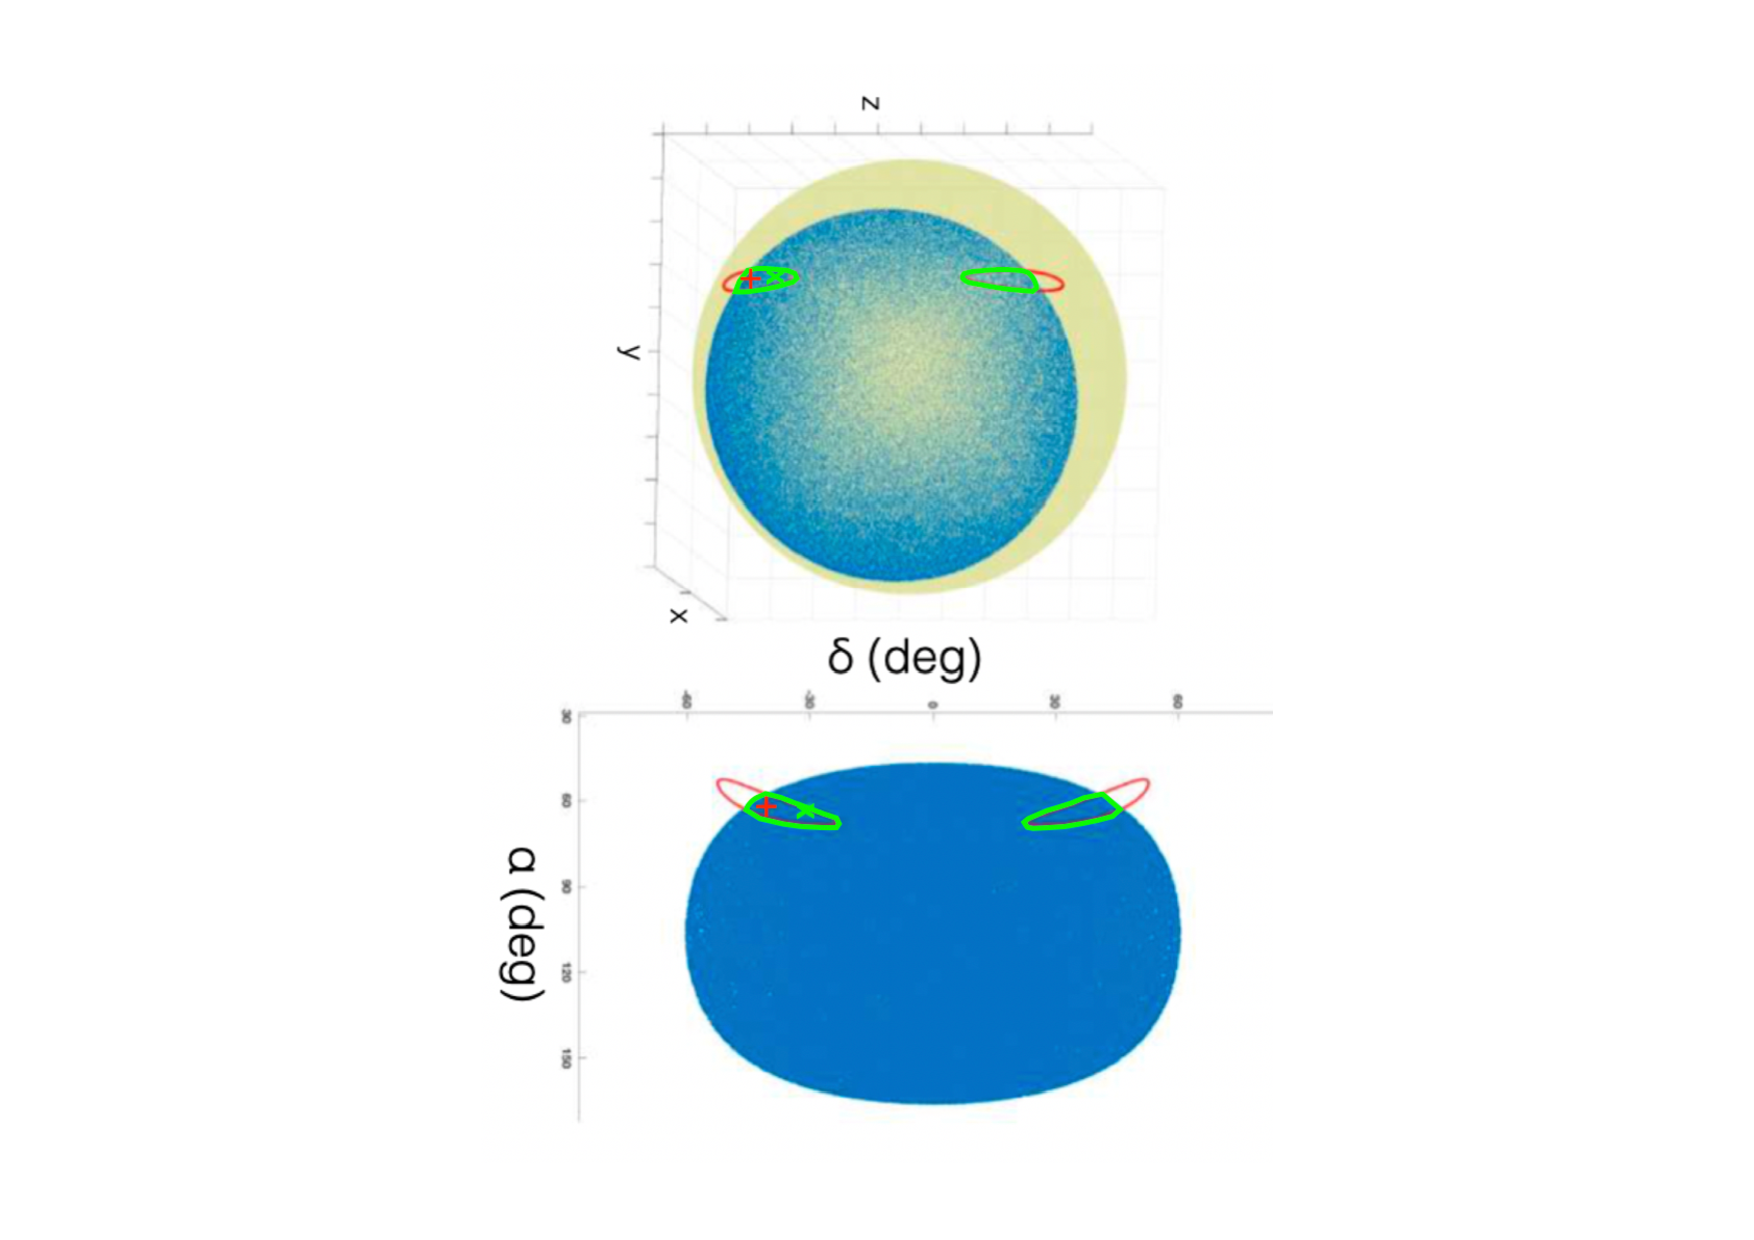
\includegraphics[scale=0.4,angle=90.0]{fig_loc_70deg}\\
a) & b)\\
\end{tabular}
\end{center}
\vspace{-3.5cm}
\caption[example] 
%>>>> use \label inside caption to get Fig. number with \ref{}
{ \label{fig:conf_reg} 
Example of GRB localization obtained by simulating a GRB with latitude < 30 deg (left panel) and latitude > 70 deg (right panel). The GRB position and best-fit position are represented with the green X-symbol and the red +-symbol, respectively.  The red contour line shows the 1$\sigma$ confidence level region associated with the best fit position. The blue-filled region represents the overlapping FoVs of the 3 satellites observing simultaneously the GRB. The light-green contour line shows the 1$\sigma$ confidence level region taking into account the FoVs of the detectors.}
\end{figure}



In Figure~\ref{fig:conf_reg} we report an example of two possible outcomes obtained from the simulations described above. Panels a) and b) the figure summarise the results of the simulation displaying the GRB real position in the plane of the sky (green X-symbol), the best-fit position of the GRB (red +symbol) and the corresponding $1\sigma$ confidence region shown both in spherical and bi-dimensional representations. Moreover, in light-green we report the positional $1\sigma$ confidence region corrected by overlapping FoVs of detectors (blue-filled region) observing simultaneously the event. Both cases describe the localisation of GRB events detected simultaneously by 3 satellites. While for the event shown in the panel a) of Figure~\ref{fig:conf_reg} the confidence region of the GRB coordinates is nearly unconstrained in the $\delta$ coordinate, panel b) describes a more favourable scenario in which the uncertainty on the GRB position is limited to a relatively small region. For the former case, we note that, although limited, two confidence regions are present but only one includes the position of the GRB. This ambiguity reflects the planar symmetry of the signal delays with respect to the satellite orbital plane. Differences between these two cases are the superposition of several aspects such as the accuracy in the determination of the time signal time delays, physical distances between the satellites and projected distances of the satellites with respect to the direction of the GRB event. Moreover, for the two cases discussed above (but also for the larger set of results obtained with the simulations) we note that the Right Ascension is always relatively well constrained, leaving the largest uncertainty in the Declination. This result is expected when considering triplets of satellites laying in the equatorial plane. Improvements in $\delta$ can be obtained by increasing the number of satellites simultaneously observing the GRB event and located in inclined plane with respect to the equatorial one.



\section{Results and Discussion}



\begin{comment}
\section{Discussion}

To obtain a realistic estimation of the accuracy that can be achieved in the measurement of the delays of the arrival times for photons emitted by GRBs in two detectors, we built a method with which we simulated several light curves of different kinds of GRBs. From a cross correlation of each couple of curves we obtained a measurement of the delay between the two signals that was obtained by fitting the peak of the cross correlation profile with an opportune function. \\
With a so large sample of GRBs events analysed, a good estimation of the accuracy in determining the delays is given by measuring how for a given typology of burst (long or short) and for each simulated area the centroids distributes around the value of the injected delay. We show the distributions obtained for the long GRB 130502327 and for the short GRB 120323507 in \autoref{fig:centroid_distribution_100_hermes_sample}. 
Each delay distribution was fitted with a Normal distribution that allowed to infer a realistic estimation of the delay injected in the simulated light curves and of the dispersion of the delay measurements with respect to the expected value, i.e. a realistic estimation of the cross correlation error E$_{cc}$ defined in \autoref{eq:sigma_pos}.
This analysis has been repeated for the whole set of areas we simulated and for both the long and short GRBs. In addition, we also compared the mean cross correlation error $<\sigma>$ obtained from the analysis of the delay distributions with the mean value $<\epsilon>$ of the error associated to the centroid obtained from the fit of the cross correlation peak region. We report the results of this analysis in \autoref{tab:tabella_Long} and \autoref{tab:tabella_Short} for the long and short data sets of GRBs.
From these results it is evident how adopting the $\epsilon$ error underestimates the error on the delay measurement via the cross correlation profile, hence resulting in an overestimation of the accuracy in the position of the GRB. In particular, the ratio $<\sigma>/<\epsilon>$ decreases with decreasing the area of the detector as a consequence of the decrement of the statistics of the data collected by smaller areas. For the same reason it is evident how the mean value of $\sigma$ increases with decreasing the detector area.\\

More precisely, it is interesting to notice the trend followed by the $\sigma$ inferred by the fit of the cross correlation profile as a function of the fluence of the GRBs for each simulated area. In \autoref{fig:sigma_vs_Fluence_Long} and \autoref{fig:sigma_vs_Fluence_Short} we report these trends for the long and short GRBs considered in our work, respectively.
From a quick comparison between the plots in the two figures it can be evinced that the high statistics that can be achieved by the long GRBs, in addition to that characterizing the higher simulated areas for the short GRBs, allows to obtain a more defined profile for the trends, due to the better constraints obtained for the delay measurement in the cross correlation profile. On the contrary, the lower areas, especially for the short GRBs, implied a scattered distribution of the data. However, in both the cases it can be inferred that the error $\sigma$ on the delay measurement decreases with increasing the fluence of the considered GRB, as a consequence of the increase in the statistics of the data. \\
We modelled these trends using a functional form as $y(x)=a+bx^k$, where $k$ is a power included between -1 and -0.001. We performed a fit for each $k$ at steps of $\delta k =1\times 10^{-4}$ for a total of 9990 fits for each simulated area and GRB typology (long or short); we chose as best-fit function the one having a $k$ for which, together with the $a$ and $b$ parameters, we obtain a minimum of the $\chi^2$. 
On average, we obtained a minimum of the $\chi^2$ for $k=-0.32$ for all the areas and both for the long and short GRBs, not considering the values of $k$ obtained for the areas 0.0125 \mq and 0.0056 \mq simulated for the short GRBs, for which we obtain a considerably flat power of -0.16 and -0.01, respectively, due to the scattered profiles in these two cases. We report the obtained fit parameters in \autoref{tab:fit_sigma_Long} and \autoref{tab:fit_sigma_Short}.


\begin{table}

\footnotesize
\centering
\begin{tabular}{|c|c|c|c|c|}
\hline
\multicolumn{1}{|c|}{    } & \multicolumn{4}{c|}{\textbf{Long GRBs}}  \\
\hline
Area & $k$ & a & b & $\chi^2 (d.o.f)$  \\
($m^2$) &  &  &  &   \\

\hline
100    & -0.2 & -56(10)$\times10^{-7}$ & 20(2)$\times10^{-6}$ & 5.4$\times10^{-10}$(98) \\
50     & -0.322 & -38(6)$\times10^{-7}$ & 29(2)$\times10^{-6}$ & 6$\times10^{-10}$(98) \\
10     & -0.216 & -134(8)$\times10^{-7}$ & 49(2)$\times10^{-6}$ & 4.5$\times10^{-10}$(98) \\
1      & -0.256 & -27(2)$\times10^{-6}$ & 133(5)$\times10^{-6}$ & 4.3$\times10^{-9}$(98) \\
0.0125 & -0.313 & -44(4)$\times10^{-5}$ & 279(10)$\times10^{-5}$ & 2$\times10^{-6}$(98) \\
0.0056 & -0.608 & -18(7)$\times10^{-5}$ & 102(4)$\times10^{-4}$ & 3$\times10^{-5}$(98) \\
\hline
\end{tabular}
\label{tab:fit_sigma_Long}
\caption{Best-fit models obtained by fitting the long GRBs $\sigma$ vs. fluence profiles with the functional form $y(x)=a+bx^k$. The errors associated to the parameters were evaluated at a confidence level of the 68\%.}
\end{table}





\begin{table}

\footnotesize
\centering
\begin{tabular}{|c|c|c|c|c|}
\hline
\multicolumn{1}{|c|}{    } & \multicolumn{4}{c|}{\textbf{Short GRBs}}  \\
\hline
Area & $k$ & a & b & $\chi^2 (d.o.f)$  \\
($m^2$) &  &  &  &   \\

\hline
100 & -0.304 & -57(11)$\times10^{-7}$ & 159(14)$\times10^{-7}$ & 8.4$\times10^{-10}$(98) \\
50 & -0.303 & -8(2)$\times10^{-6}$ & 23(2)$\times10^{-6}$ & 2$\times10^{-9}$(98) \\
10 & -0.325 & -17(3)$\times10^{-6}$ & 49(4)$\times10^{-6}$ & 8$\times10^{-9}$(98) \\
1 & -0.327 & -56(11)$\times10^{-6}$ & 160(14)$\times10^{-6}$ & 1$\times10^{-7}$(98) \\
0.0125 & -0.164 & -0.011(3) & 0.018(3) & 0.002(98) \\
0.0056 & -0.010 & -0.50(14) & 0.52(15) & 0.02(98) \\
\hline
\end{tabular}
\label{tab:fit_sigma_Short}
\caption{Best-fit models obtained by fitting the short GRBs $\sigma$ vs. fluence profiles with the functional form $y(x)=a+bx^k$. The errors associated to the parameters were evaluated at a confidence level of the 68\%.}
\end{table}










\begin{figure*}[h!]
\centering
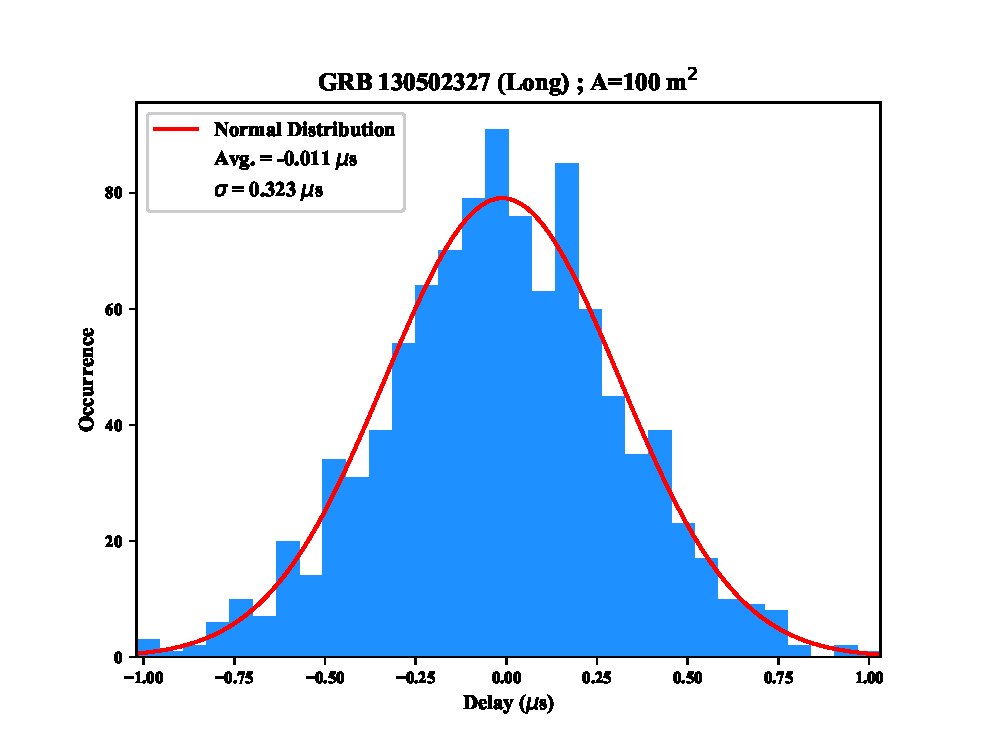
\includegraphics[scale=0.5,angle=0]{fig/distribution_long_100.eps}
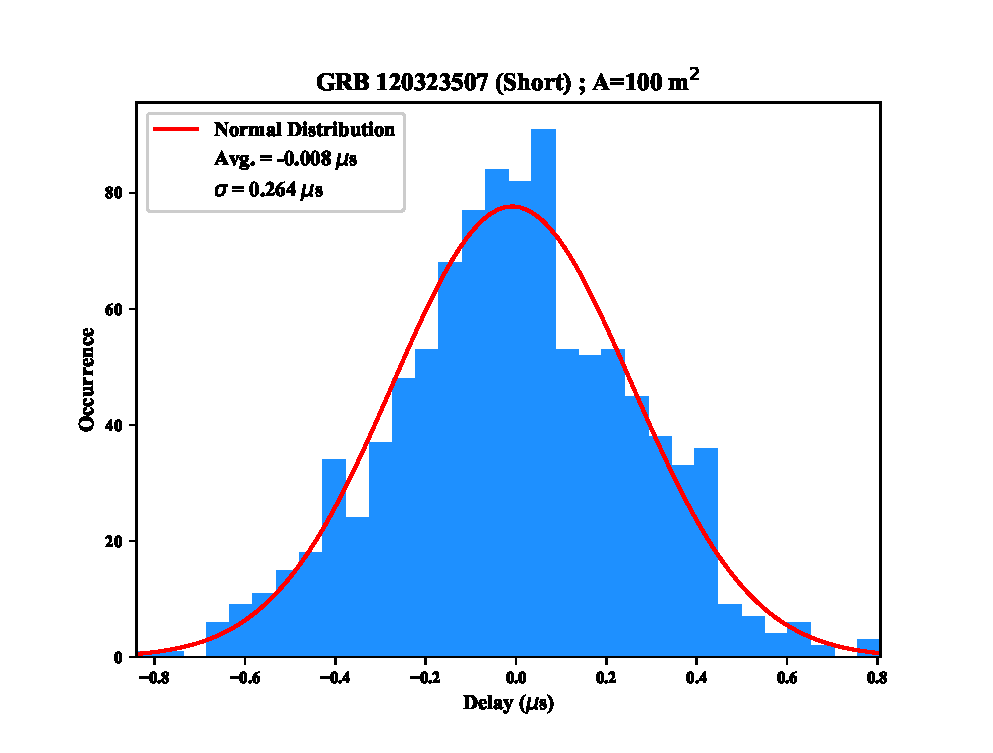
\includegraphics[scale=0.5,angle=0]{fig/distribution_short_100.eps}\\
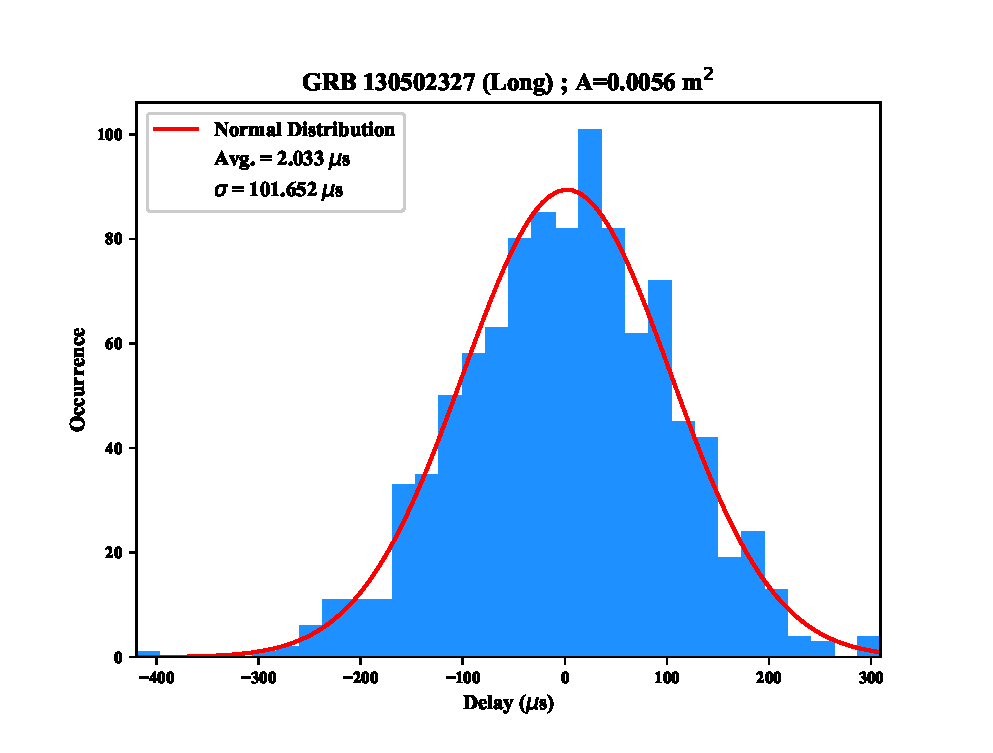
\includegraphics[scale=0.5,angle=0]{fig/distribution_long_56.eps}
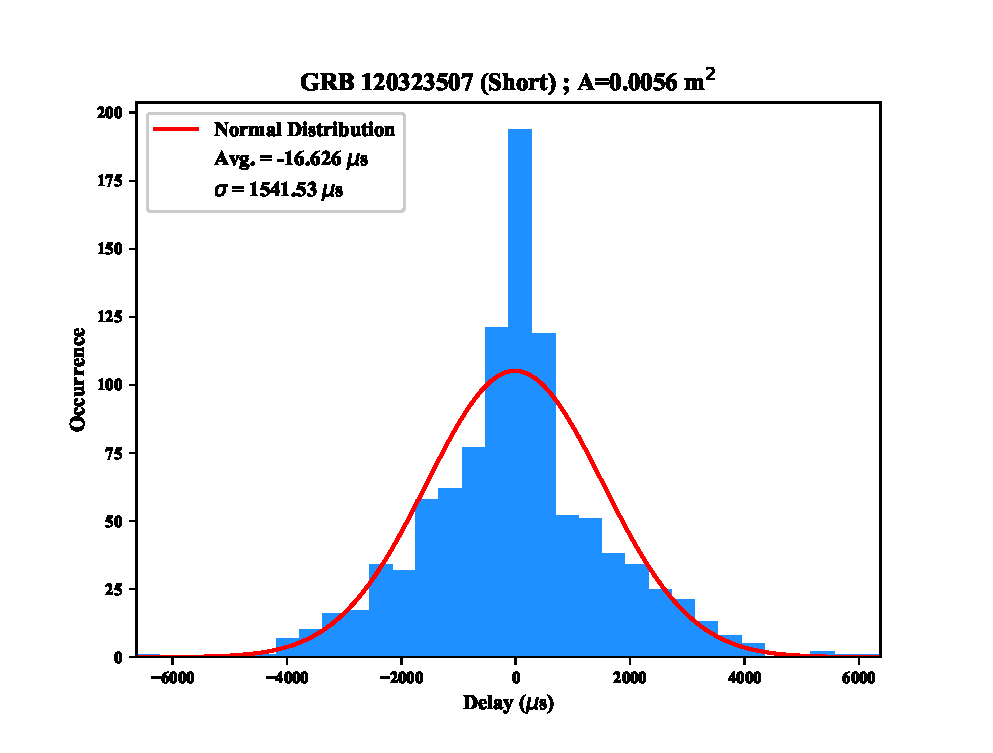
\includegraphics[scale=0.5,angle=0]{fig/distribution_short_56.eps}

\caption{Distributions of the delays obtained for the long GRB 130502327 (left column) and the short GRB 120323507 (right column). For each burst we show a comparison between the results obtained for a simulated area of 100 m$^2$ (on the top) and of 0.0056 m$^2$ (on the bottom).}
\label{fig:centroid_distribution_100_hermes_sample}
\end{figure*}














\begin{table*}

\footnotesize
\centering
\begin{tabular}{|c|c|c|c|c|}
\hline
 \multicolumn{1}{|c|}{    } & \multicolumn{4}{c|}{\textbf{Short GRBs}}  \\
\hline
Area & $\sigma_{min}$ & $\sigma_{max}$ & $<\sigma>$ & $<\sigma>$/$<\epsilon>$  \\
($m^2$) &  &  &  &   \\

\hline
100 & 5.974907063724057e-08 & 1.8347673286588637e-05 & 6.534330112671629e-06 & 7.3457365782627235 \\
50 & 8.327817977413326e-08 & 2.8146661479250482e-05 & 9.21619292355443e-06 & 6.200167445616318 \\
10 & 1.867258872028386e-07 & 6.102888687738298e-05 & 2.0331103734181935e-05 & 6.701879256463874 \\
1 & 5.771539436685253e-07 & 0.00021081777428695462 & 6.453042063262608e-05 & 5.039805652851995 \\
0.0125 & 9.560084714842066e-06 & 0.025972208446171898 & 0.004584209602272932 & 4.294325462320192 \\
0.0056 & 1.9398674274012946e-05 & 0.0787462424572527 & 0.01360441039839945 & 4.811604623009573 \\
\hline
\end{tabular}
\label{tab:tabella_Short}
\caption{Resume of the results obtained from the simulation of a sample of 100 Short GRBs from the Fermi/GBM archive as a function of the simulated collecting area.}
\end{table*}




\begin{table*}

\footnotesize
\centering
\begin{tabular}{|c|c|c|c|c|}
\hline
 \multicolumn{1}{|c|}{    } & \multicolumn{4}{c|}{\textbf{Long GRBs}}\\
\hline
Area & $\sigma_{min}$ & $\sigma_{max}$ & $<\sigma>$ & $<\sigma>$/$<\epsilon>$\\
($m^2$) &  &  &  &   \\

\hline
100 & 1.2288202791919088e-07 & 1.3893084036386532e-05 & 4.421738574898745e-06 & 5.163571094402115 \\
50 & 1.7357168814420108e-07 & 2.0104233385850118e-05 & 5.669313287935561e-06 & 3.2135421748743354  \\
10 & 3.987123355230972e-07 & 2.5728427221454894e-05 & 9.320900692181446e-06 & 3.2093913438856703 \\
1 & 1.3132966330242298e-06 & 7.713557028223853e-05 & 2.6879835390663862e-05 & 2.8811619807648956 \\
0.0125 & 1.798680374494856e-05 & 0.001739569989617569 & 0.0004975834853598062 & 1.3351867706734453 \\
0.0056 & 3.4300685103588634e-05 & 0.0063206606110297586 & 0.001209711899944309 & 1.252797733846769 \\
\hline
\end{tabular}
\label{tab:tabella_Long}
\caption{Resume of the results obtained from the simulation of a sample of 100 Long GRBs from the Fermi/GBM archive as a function of the simulated collecting area.}
\end{table*}



%%%%%%%%%%%%%%%%%%%%%%    Serie di Plot   %%%%%%%%%%%%%%%%%%%%%%%%%%

%\begin{landscape}
\begin{figure*}[h!]
\centering
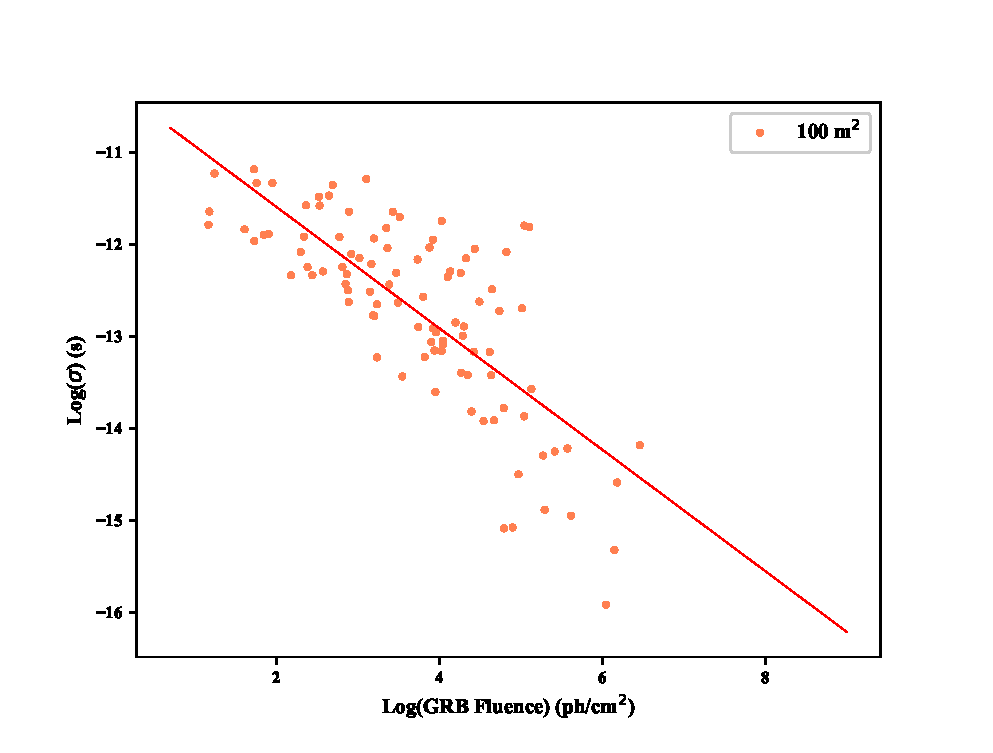
\includegraphics[scale=0.5,angle=0]{fig/LONG/sigma_vs_fluence_100.eps}
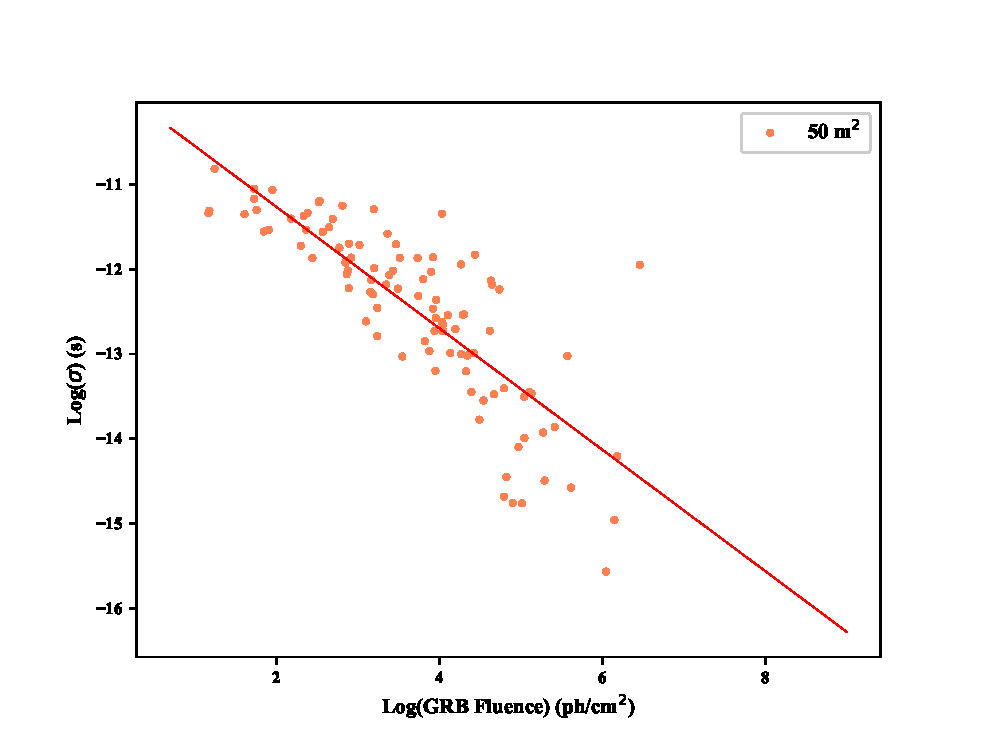
\includegraphics[scale=0.5,angle=0]{fig/LONG/sigma_vs_fluence_50.eps}\\
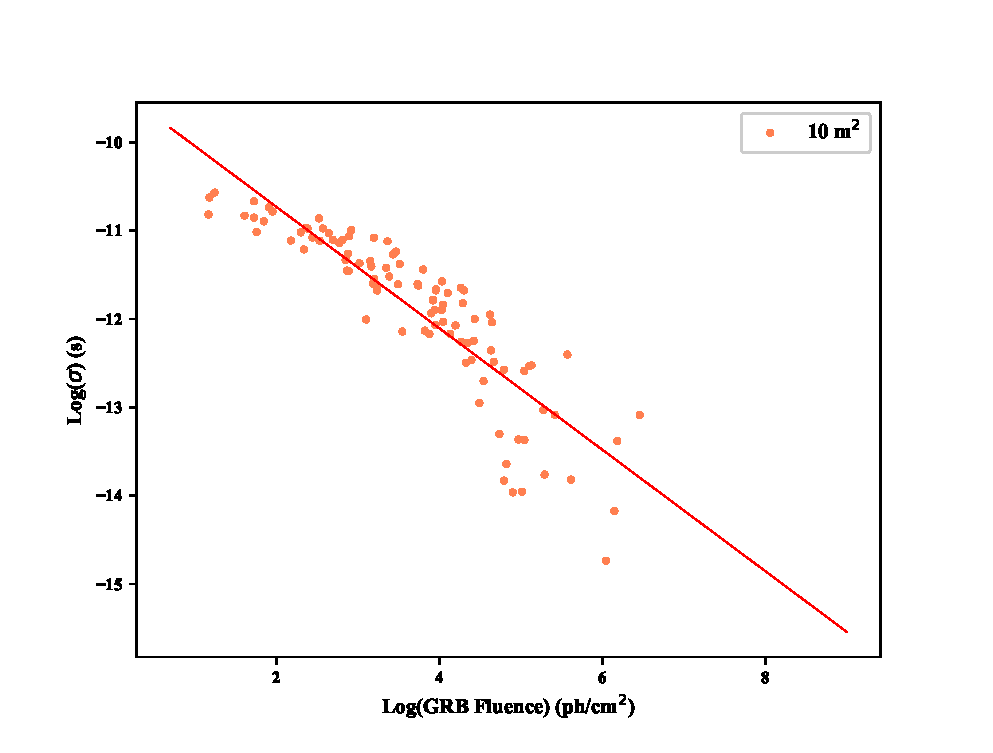
\includegraphics[scale=0.5,angle=0]{fig/LONG/sigma_vs_fluence_10.eps}
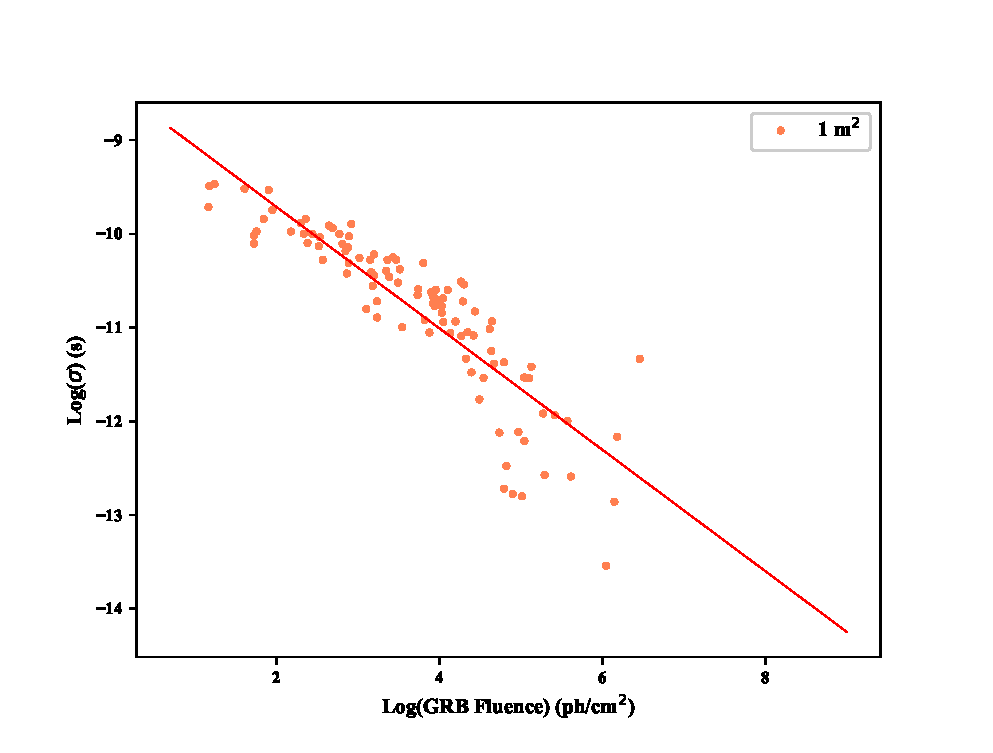
\includegraphics[scale=0.5,angle=0]{fig/LONG/sigma_vs_fluence_1.eps}\\
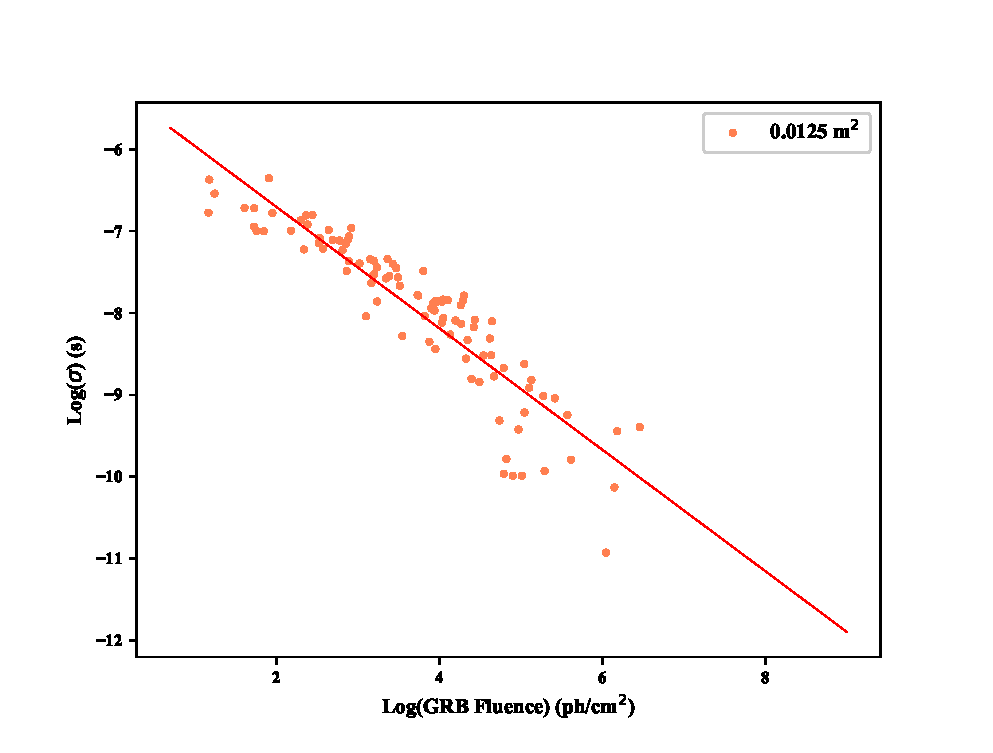
\includegraphics[scale=0.5,angle=0]{fig/LONG/sigma_vs_fluence_0.0125.eps}
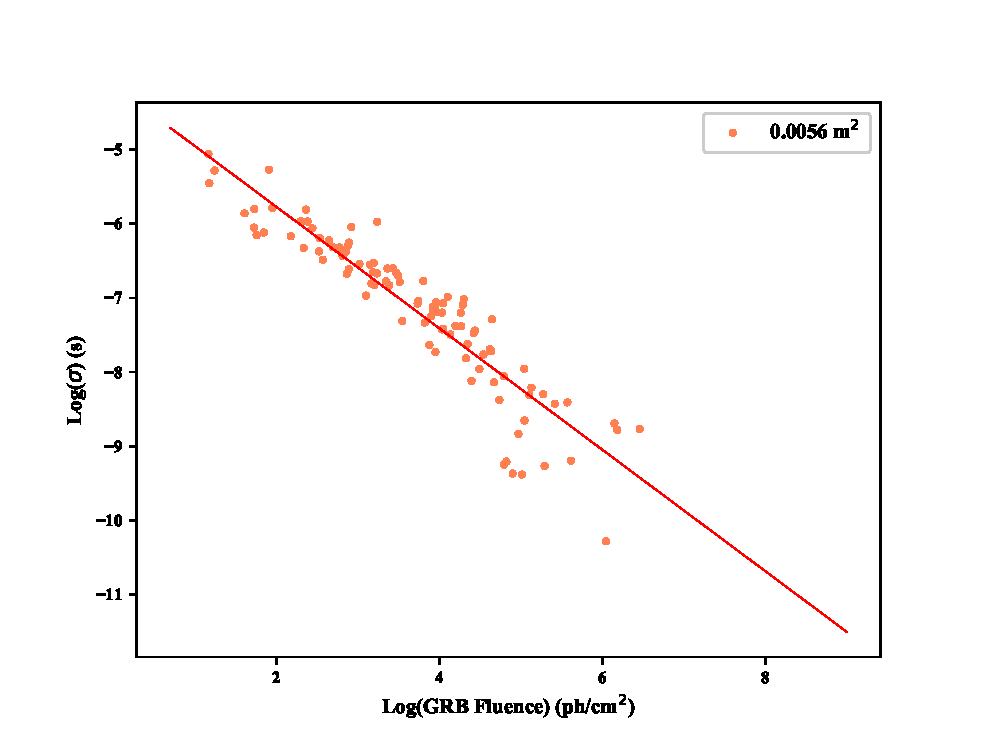
\includegraphics[scale=0.5,angle=0]{fig/LONG/sigma_vs_fluence_0.0056.eps}\\

\caption{$\sigma$ of the centroids distribution obtained from the cross correlation curves of the long GRBs, as a function of the GRB fluence for each simulated area. The red solid lines represent the best-fit functions $y(x)=a+bx^{k}$, where $k$ is the power that minimizes the $\chi^2$, together with the parameters $a$ and $b$  (see \autoref{tab:fit_sigma_Long} and \autoref{tab:fit_sigma_Short} for the parameters obtained for the long and short GRBs, respectively).}
\label{fig:sigma_vs_Fluence_Long}
\end{figure*}
%\end{landscape}




%\begin{landscape}
\begin{figure*}[h!]
\centering
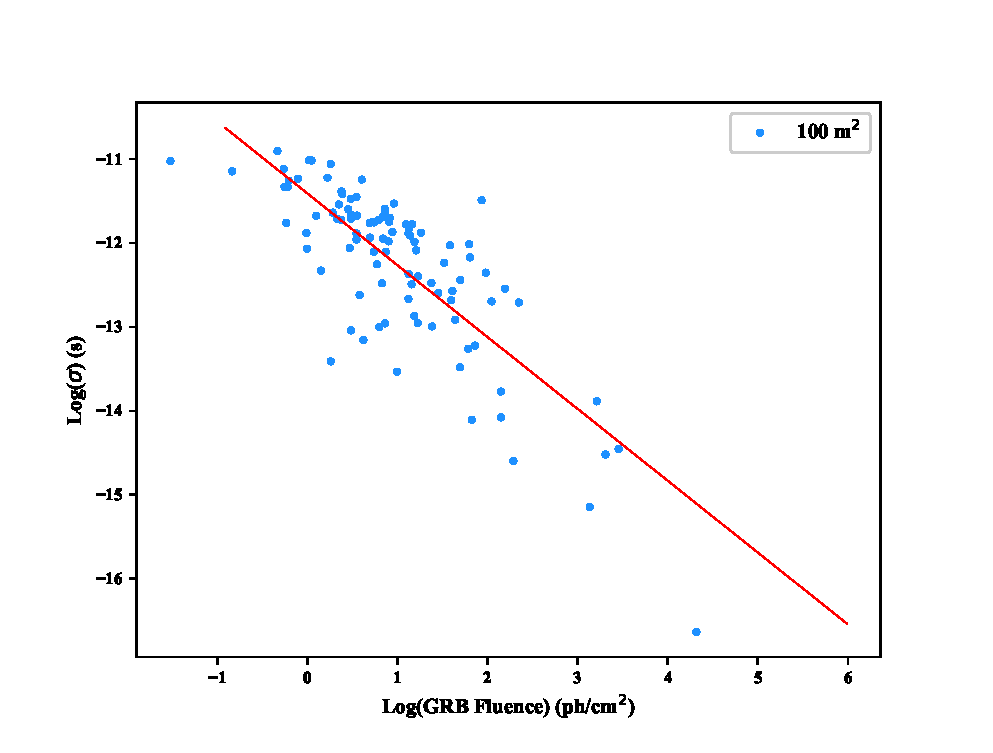
\includegraphics[scale=0.5,angle=0]{fig/SHORT/sigma_vs_fluence_100.eps}
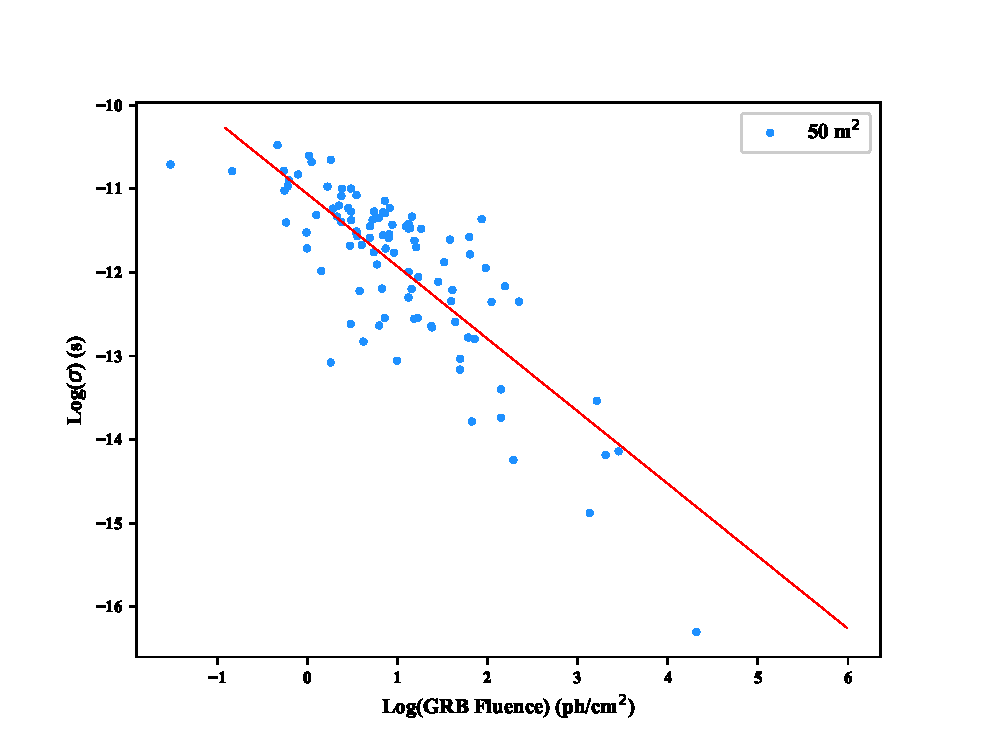
\includegraphics[scale=0.5,angle=0]{fig/SHORT/sigma_vs_fluence_50.eps}\\
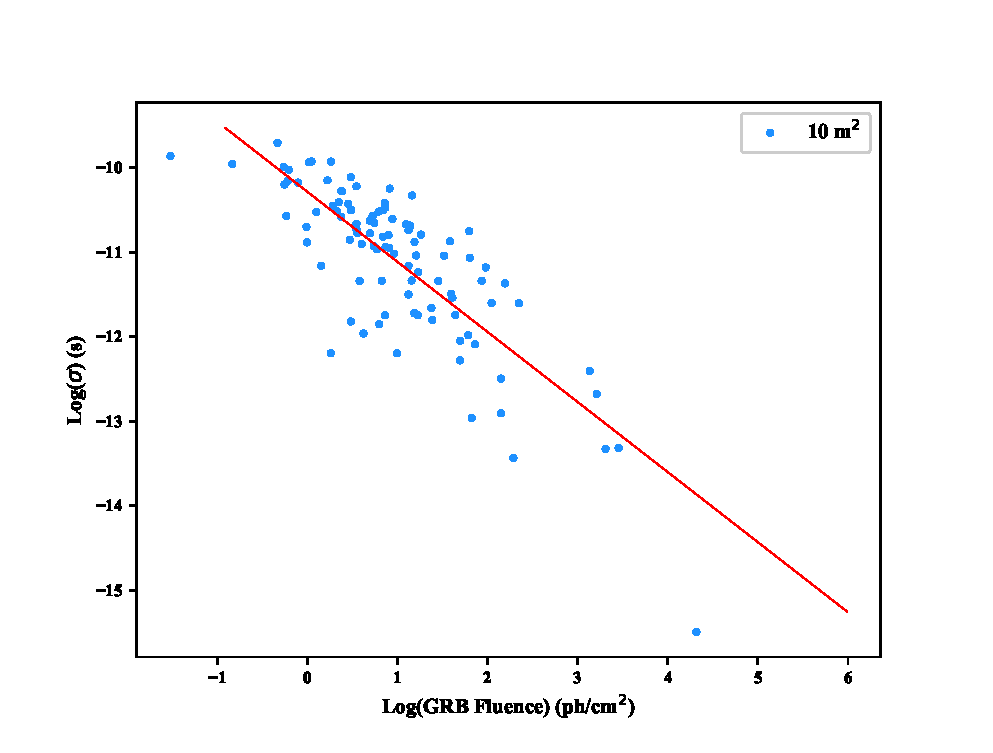
\includegraphics[scale=0.5,angle=0]{fig/SHORT/sigma_vs_fluence_10.eps}
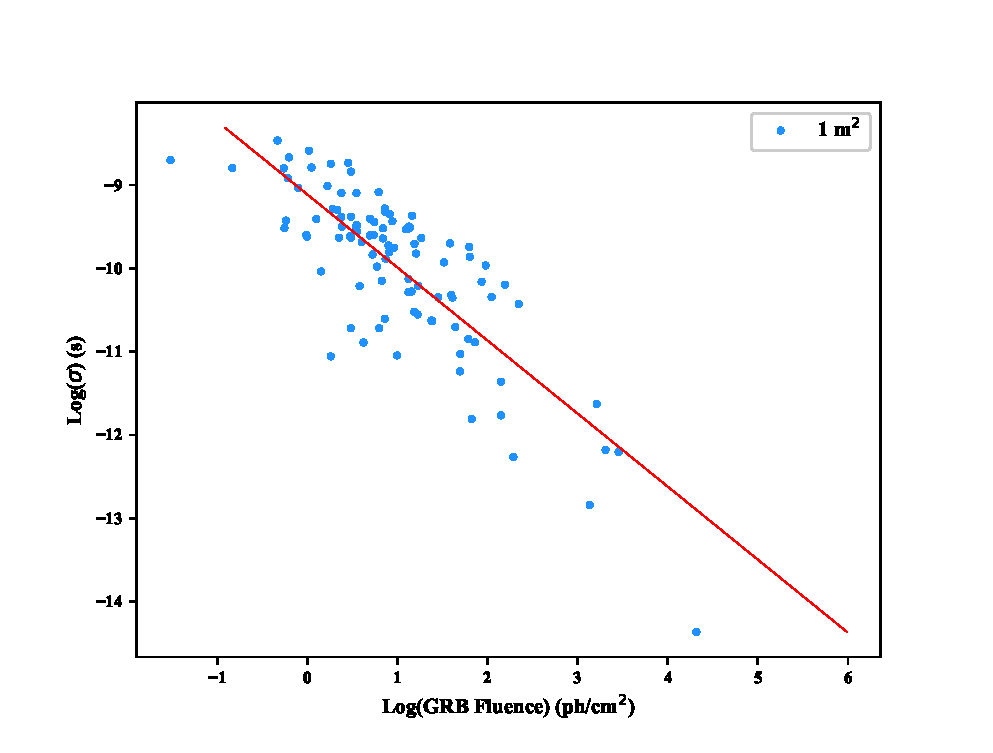
\includegraphics[scale=0.5,angle=0]{fig/SHORT/sigma_vs_fluence_1.eps}\\
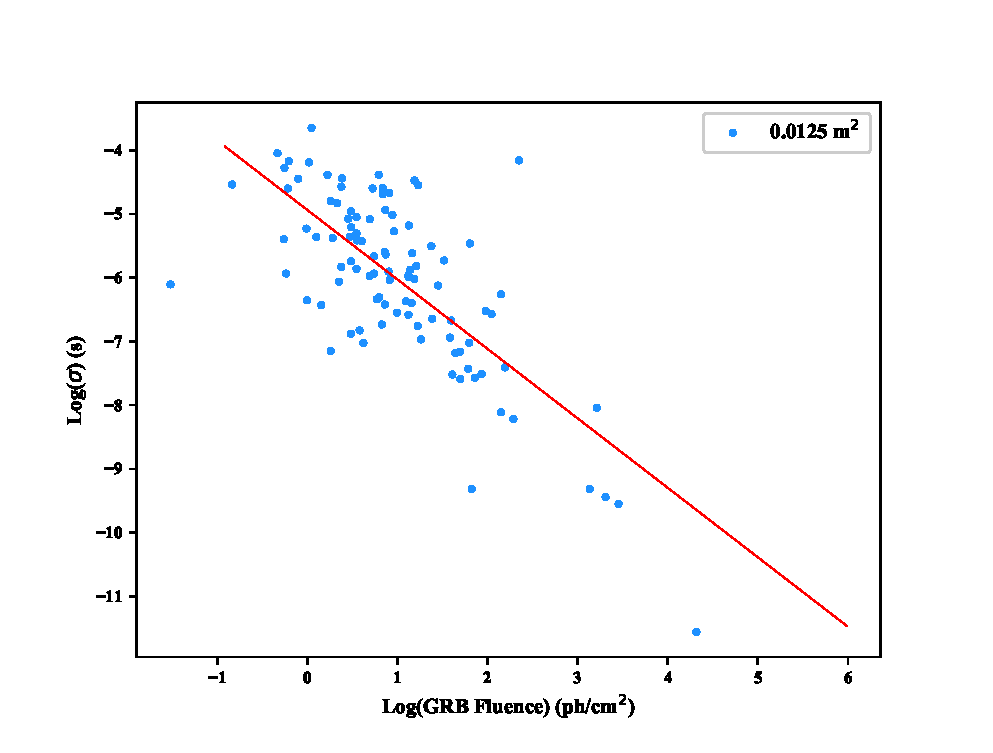
\includegraphics[scale=0.5,angle=0]{fig/SHORT/sigma_vs_fluence_0.0125.eps}
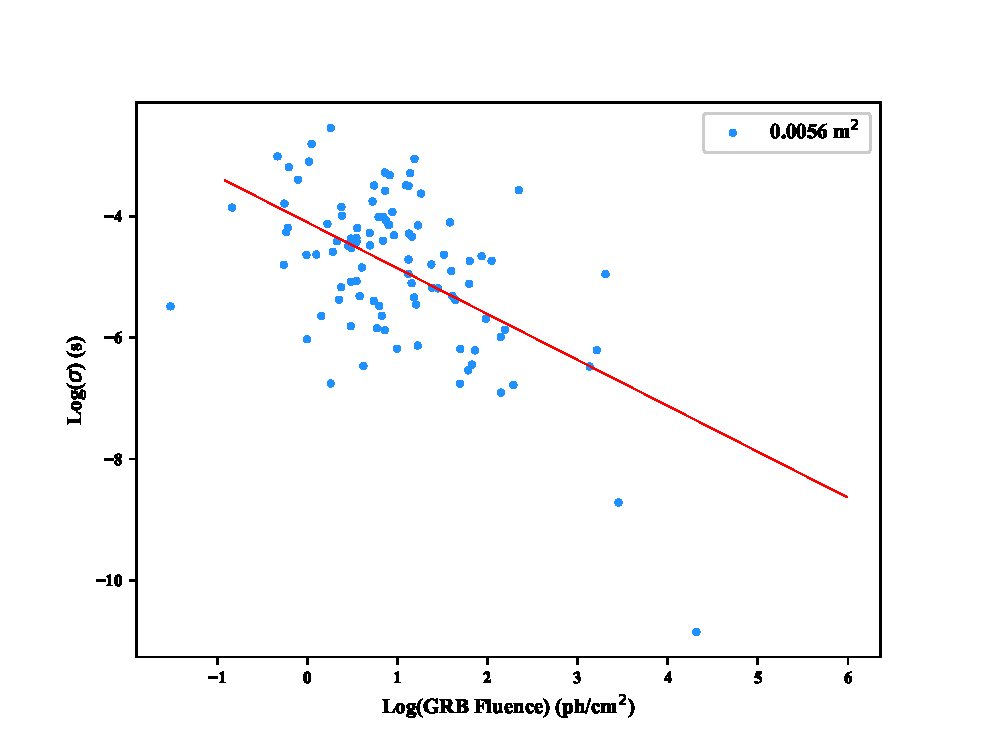
\includegraphics[scale=0.5,angle=0]{fig/SHORT/sigma_vs_fluence_0.0056.eps}\\

\caption{$\sigma$ of the centroids distribution obtained from the cross correlation curves of the short GRBs, as a function of the GRB fluence for each simulated area. The red solid lines represent the best-fit functions $y(x)=a+bx^{k}$, where $k$ is the power that minimizes the $\chi^2$, together with the parameters $a$ and $b$  (see \autoref{tab:fit_sigma_Long} and \autoref{tab:fit_sigma_Short} for the parameters obtained for the long and short GRBs, respectively).}
\label{fig:sigma_vs_Fluence_Short}
\end{figure*}
%\end{landscape}







%\begin{landscape}
\begin{figure*}[h!]
\centering
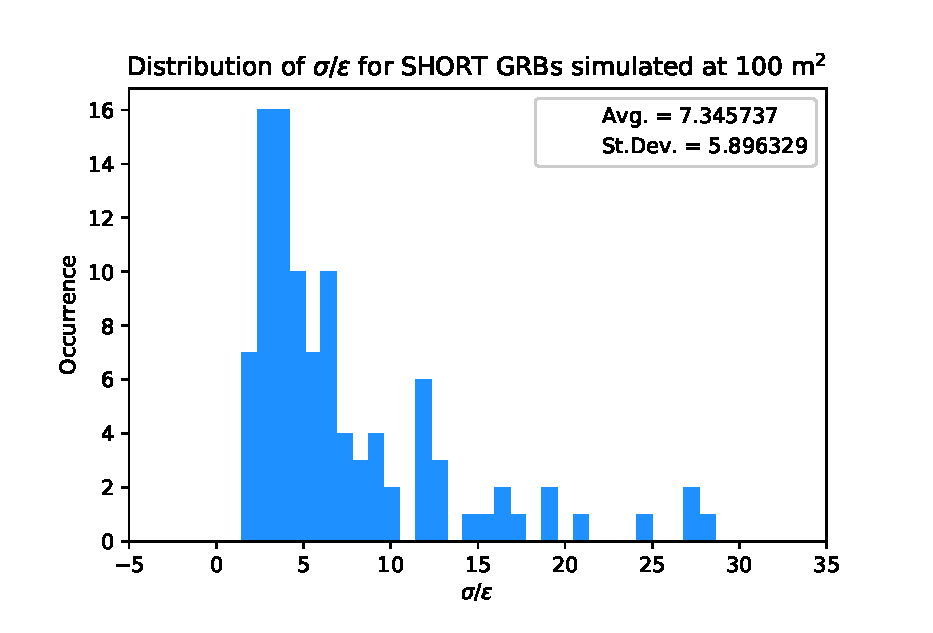
\includegraphics[scale=0.5,angle=0]{fig/SHORT/ratio_distrib_100.eps}
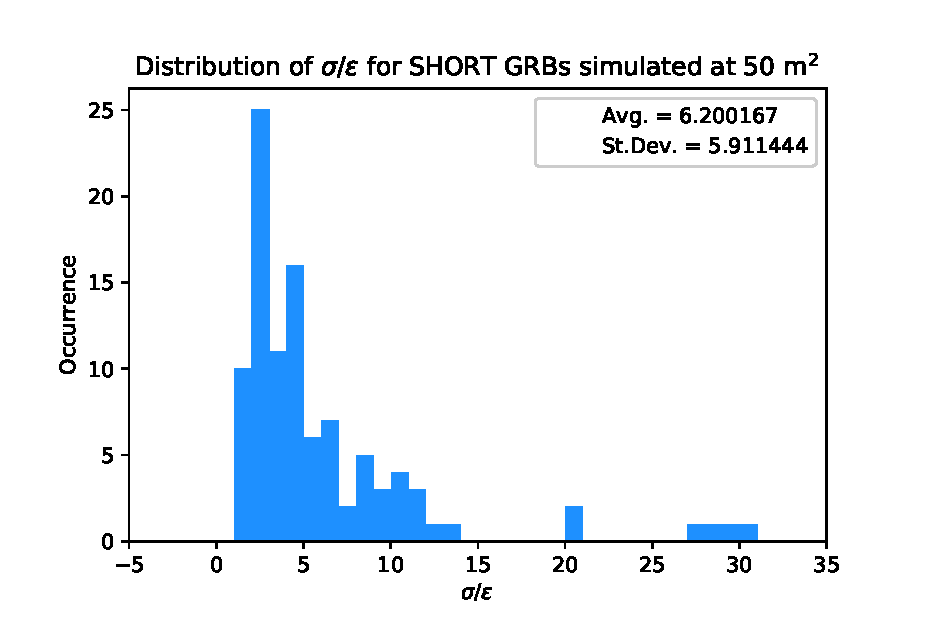
\includegraphics[scale=0.5,angle=0]{fig/SHORT/ratio_distrib_50.eps}\\
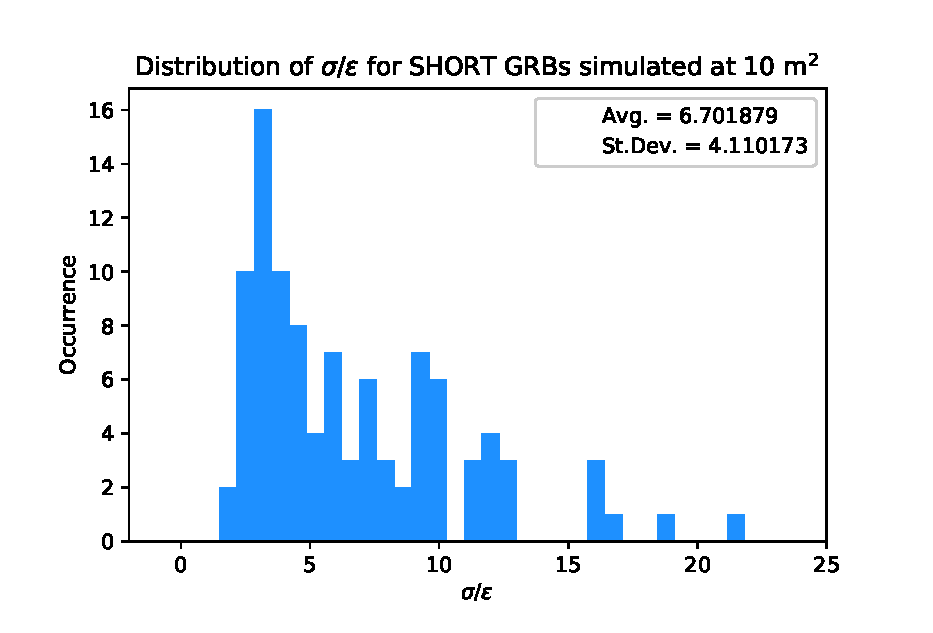
\includegraphics[scale=0.5,angle=0]{fig/SHORT/ratio_distrib_10.eps}
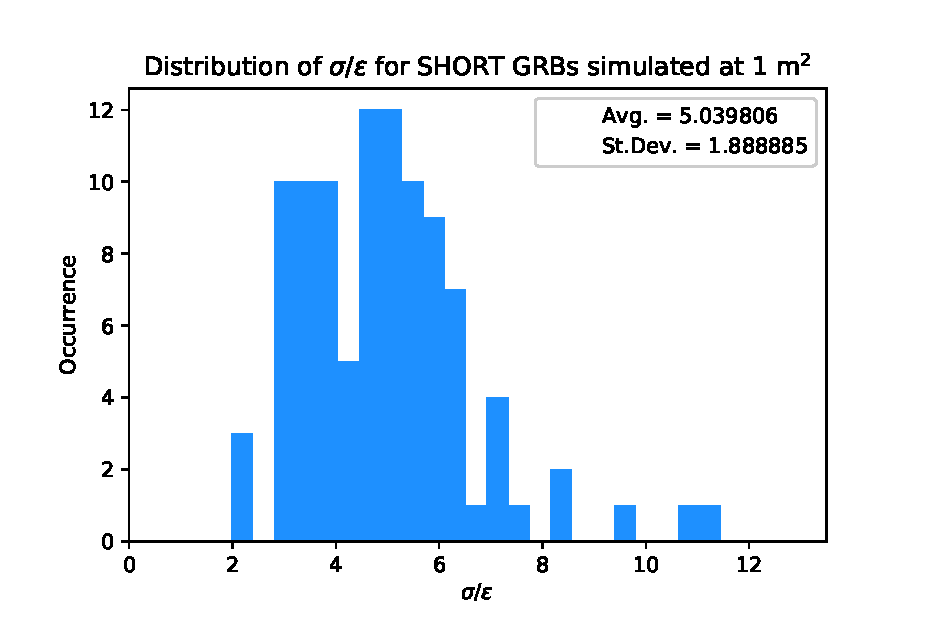
\includegraphics[scale=0.5,angle=0]{fig/SHORT/ratio_distrib_1.eps}\\
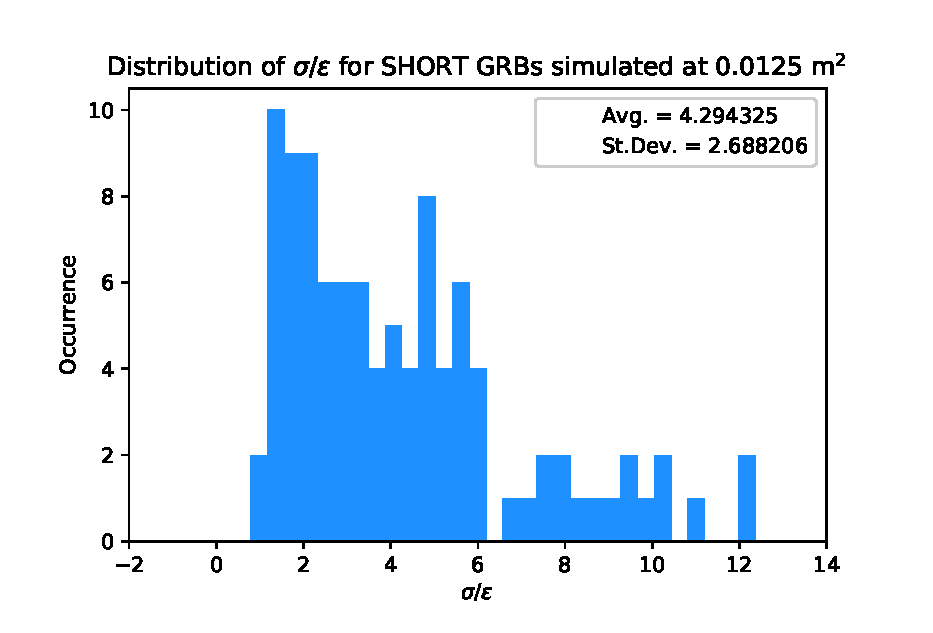
\includegraphics[scale=0.5,angle=0]{fig/SHORT/ratio_distrib_0.0125.eps}
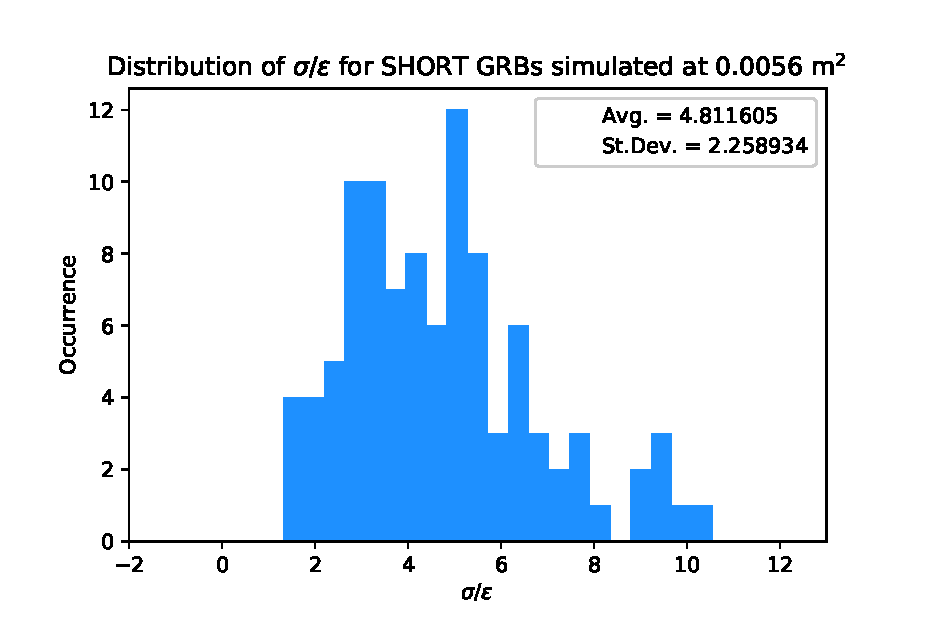
\includegraphics[scale=0.5,angle=0]{fig/SHORT/ratio_distrib_0.0056.eps}\\

\caption{...}
\label{fig:ratio_distribution_Short}
\end{figure*}
%\end{landscape}



%\begin{landscape}
\begin{figure*}[h!]
\centering
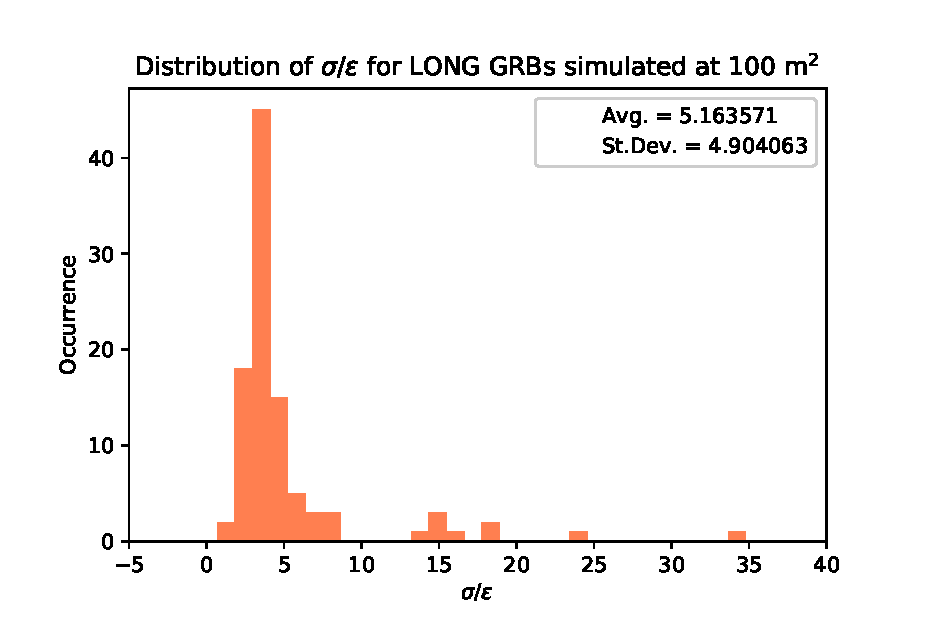
\includegraphics[scale=0.5,angle=0]{fig/LONG/ratio_distrib_100.eps}
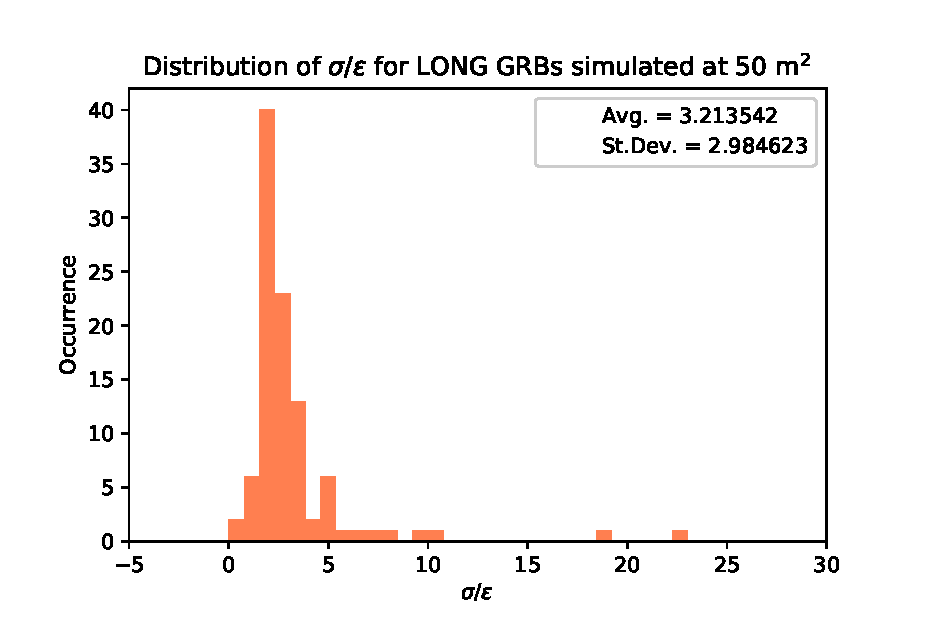
\includegraphics[scale=0.5,angle=0]{fig/LONG/ratio_distrib_50.eps}\\
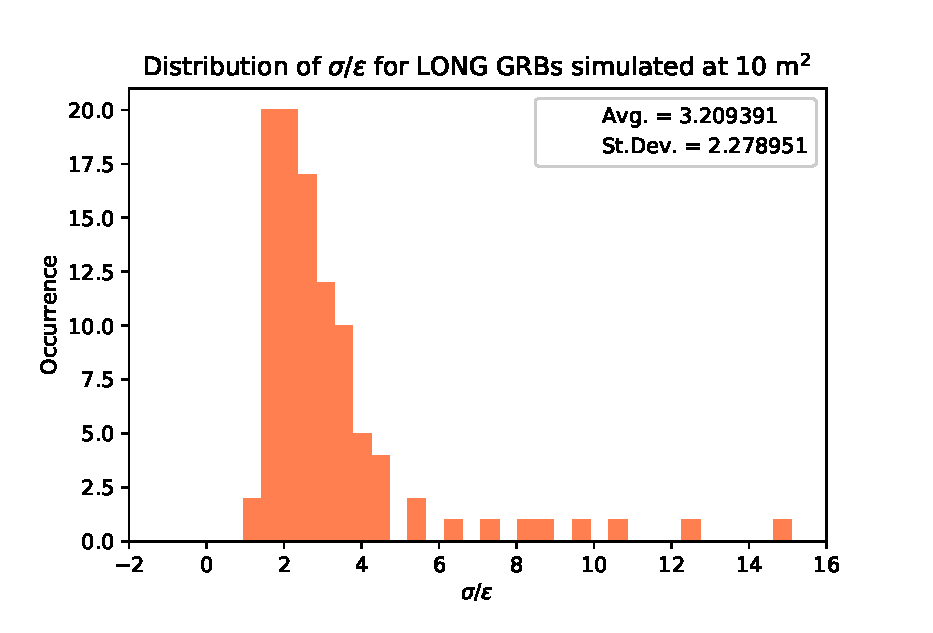
\includegraphics[scale=0.5,angle=0]{fig/LONG/ratio_distrib_10.eps}
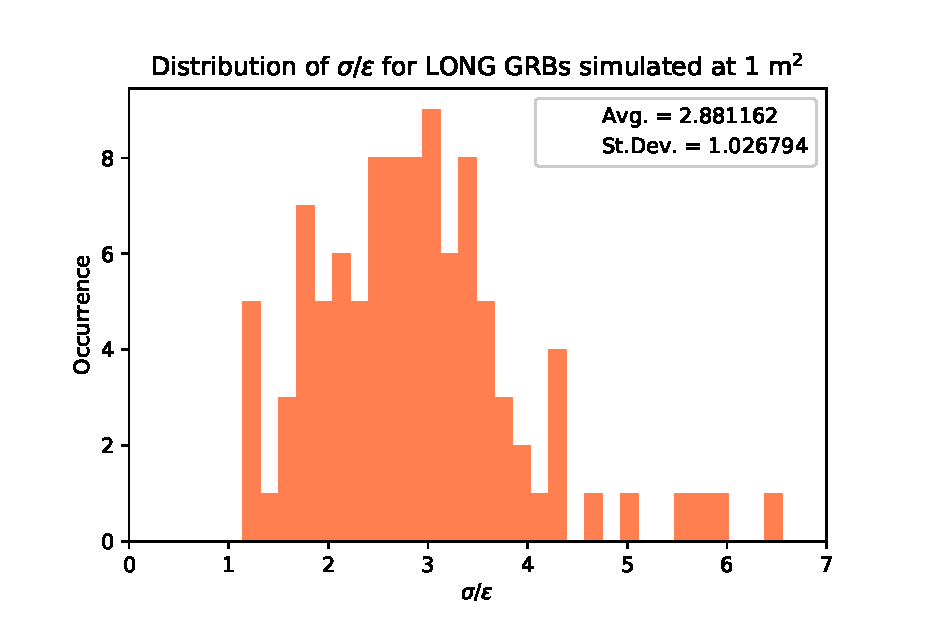
\includegraphics[scale=0.5,angle=0]{fig/LONG/ratio_distrib_1.eps}\\
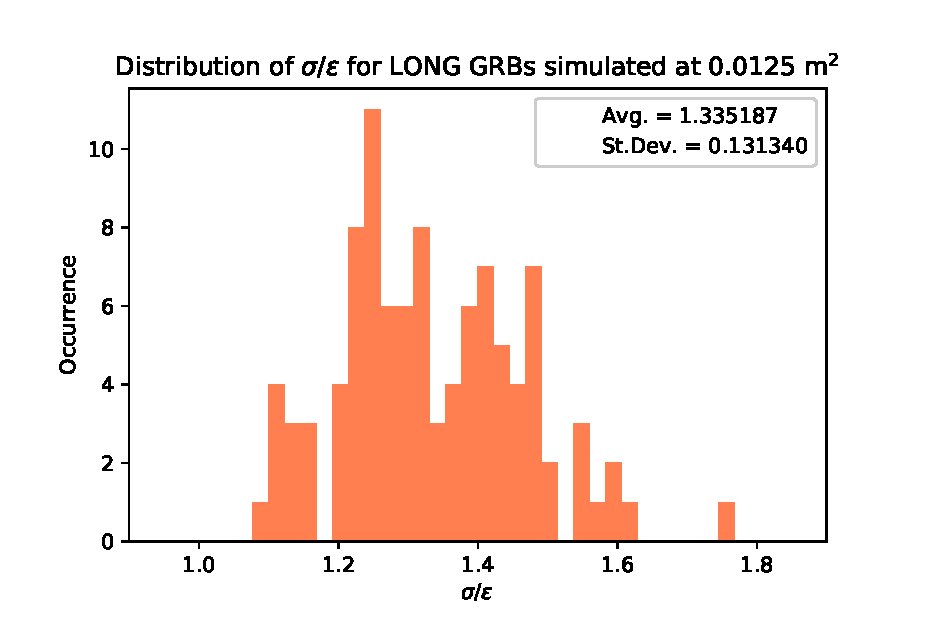
\includegraphics[scale=0.5,angle=0]{fig/LONG/ratio_distrib_0.0125.eps}
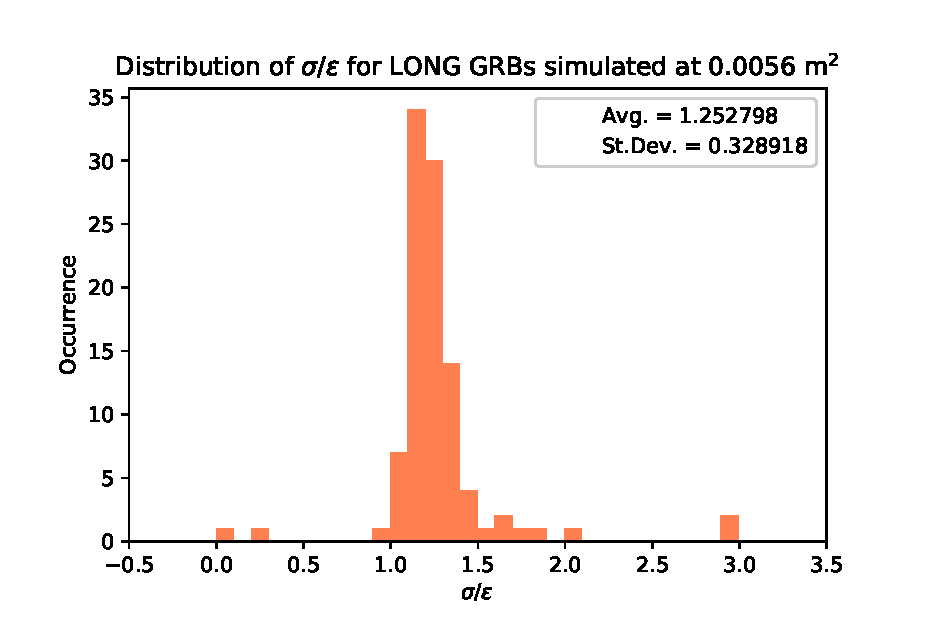
\includegraphics[scale=0.5,angle=0]{fig/LONG/ratio_distrib_0.0056.eps}\\

\caption{...}
\label{fig:ratio_distribution_Long}
\end{figure*}
%\end{landscape}



\begin{figure*}[h!]
\centering
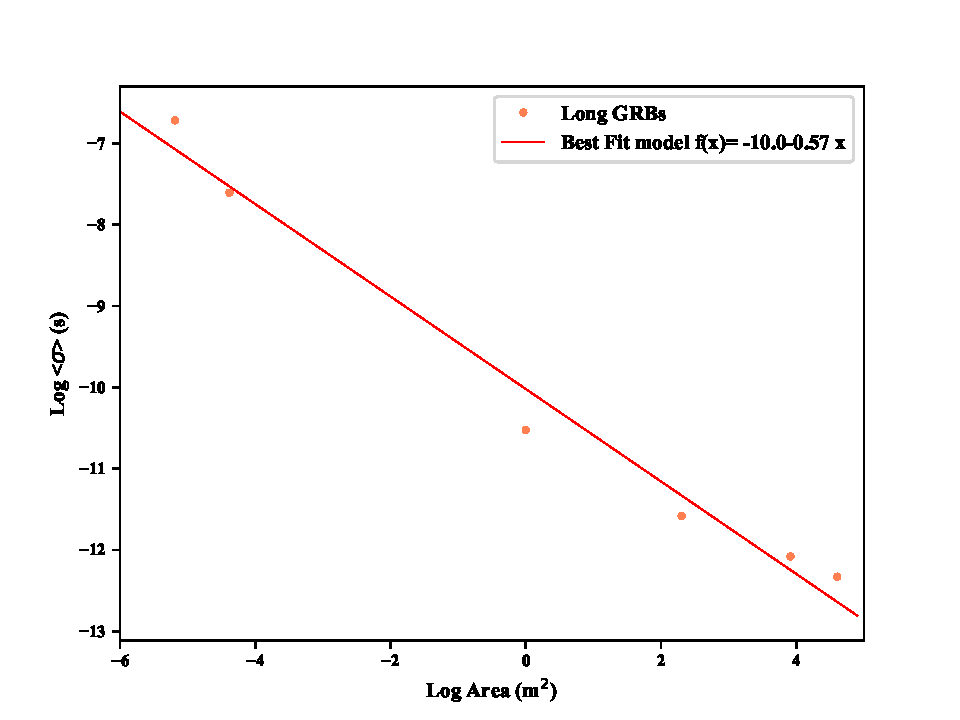
\includegraphics[scale=0.5,angle=0]{fig/sigma_vs_area_Long.pdf}
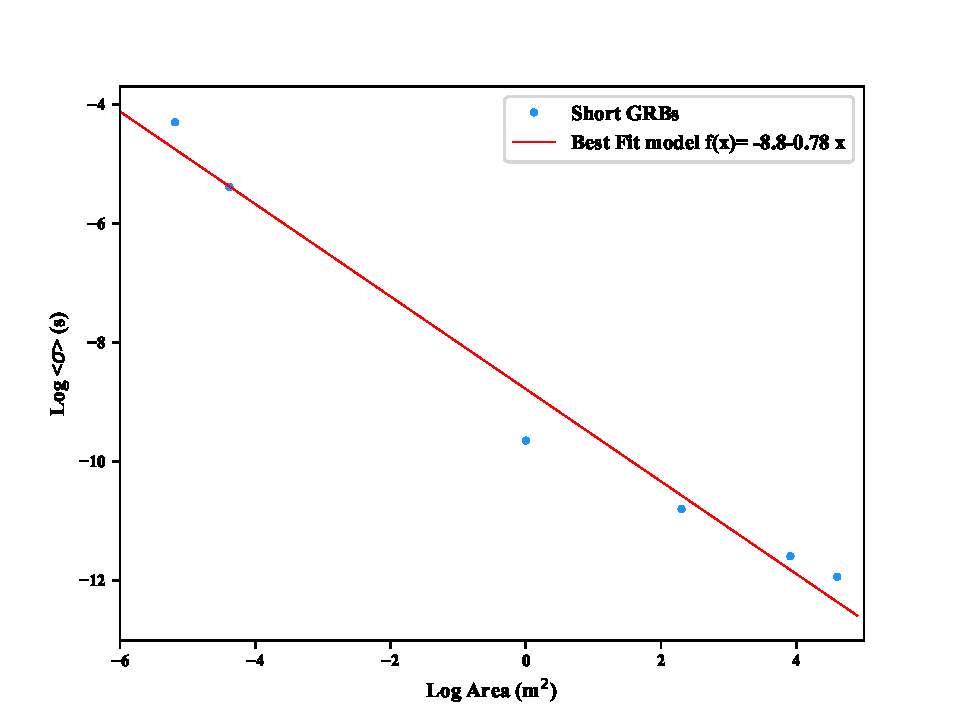
\includegraphics[scale=0.5,angle=0]{fig/sigma_vs_area_Short.pdf}


\caption{Trend of the mean value of the $\sigma$ obtained for each simulated area as a function of the area of the detector. We also report the best-fit linear function (red solid line) superimposed in each plot.}
\label{fig:sigmed_vs_area}
\end{figure*}

\end{comment}


\begin{comment}
\begin{table}[ht]
\caption{Fonts sizes to be used for various parts of the manuscript.  Table captions should be centered above the table.  When the caption is too long to fit on one line, it should be justified to the right and left margins of the body of the text.} 
\label{tab:fonts}
\begin{center}       
\begin{tabular}{|l|l|} %% this creates two columns
%% |l|l| to left justify each column entry
%% |c|c| to center each column entry
%% use of \rule[]{}{} below opens up each row
\hline
\rule[-1ex]{0pt}{3.5ex}  Article title & 16 pt., bold, centered  \\
\hline
\rule[-1ex]{0pt}{3.5ex}  Author names and affiliations & 12 pt., normal, centered   \\
\hline
\rule[-1ex]{0pt}{3.5ex}  Keywords & 10 pt., normal, left justified   \\
\hline
\rule[-1ex]{0pt}{3.5ex}  Abstract Title & 11 pt., bold, centered   \\
\hline
\rule[-1ex]{0pt}{3.5ex}  Abstract body text & 10 pt., normal, justified   \\
\hline
\rule[-1ex]{0pt}{3.5ex}  Section heading & 11 pt., bold, centered (all caps)  \\
\hline
\rule[-1ex]{0pt}{3.5ex}  Subsection heading & 11 pt., bold, left justified  \\
\hline
\rule[-1ex]{0pt}{3.5ex}  Sub-subsection heading & 10 pt., bold, left justified  \\
\hline
\rule[-1ex]{0pt}{3.5ex}  Normal text & 10 pt., normal, justified  \\
\hline
\rule[-1ex]{0pt}{3.5ex}  Figure and table captions & \, 9 pt., normal \\
\hline
\rule[-1ex]{0pt}{3.5ex}  Footnote & \, 9 pt., normal \\
\hline 
\rule[-1ex]{0pt}{3.5ex}  Reference Heading & 11 pt., bold, centered   \\
\hline
\rule[-1ex]{0pt}{3.5ex}  Reference Listing & 10 pt., normal, justified   \\
\hline
\end{tabular}
\end{center}
\end{table} 

\begin{table}[ht]
\caption{Margins and print area specifications.} 
\label{tab:Paper Margins}
\begin{center}       
\begin{tabular}{|l|l|l|} 
\hline
\rule[-1ex]{0pt}{3.5ex}  Margin & A4 & Letter  \\
\hline
\rule[-1ex]{0pt}{3.5ex}  Top margin & 2.54 cm & 1.0 in.   \\
\hline
\rule[-1ex]{0pt}{3.5ex}  Bottom margin & 4.94 cm & 1.25 in.  \\
\hline
\rule[-1ex]{0pt}{3.5ex}  Left, right margin & 1.925 cm & .875 in.  \\
\hline
\rule[-1ex]{0pt}{3.5ex}  Printable area & 17.15 x 22.23 cm & 6.75 x 8.75 in.  \\
\hline 
\end{tabular}
\end{center}
\end{table}

LaTeX margins are related to the document's paper size. The paper size is by default set to USA letter paper. To format a document for A4 paper, the first line of this LaTeX source file should be changed to \verb|\documentclass[a4paper]{spie}|.   

Authors are encouraged to follow the principles of sound technical writing, as described in Refs.~\citenum{Alred03} and \citenum{Perelman97}, for example.  Many aspects of technical writing are addressed in the {\em AIP Style Manual}, published by the American Institute of Physics.  It is available on line at \url{https://publishing.aip.org/authors}. A spelling checker is helpful for finding misspelled words. 

An author may use this LaTeX source file as a template by substituting his/her own text in each field.  This document is not meant to be a complete guide on how to use LaTeX.  For that, please see the list of references at \url{http://latex-project.org/guides/} and for an online introduction to LaTeX please see \citenum{Lees-Miller-LaTeX-course-1}. 
\end{comment}











\begin{comment}


\section{FORMATTING OF MANUSCRIPT COMPONENTS}

This section describes the normal structure of a manuscript and how each part should be handled.  The appropriate vertical spacing between various parts of this document is achieved in LaTeX through the proper use of defined constructs, such as \verb|\section{}|.  In LaTeX, paragraphs are separated by blank lines in the source file. 

At times it may be desired, for formatting reasons, to break a line without starting a new paragraph.  This situation may occur, for example, when formatting the article title, author information, or section headings.  Line breaks are inserted in LaTeX by entering \verb|\\| or \verb|\linebreak| in the LaTeX source file at the desired location.  


\subsection{Title and Author Information}
\label{sec:title}

The article title appears centered at the top of the first page.  The title font is 16 point, bold.  The rules for capitalizing the title are the same as for sentences; only the first word, proper nouns, and acronyms should be capitalized.  Avoid using acronyms in the title.  Keep in mind that people outside your area of expertise might read your article. At the first occurrence of an acronym, spell it out, followed by the acronym in parentheses, e.g., noise power spectrum (NPS). 

The author list is in 12-pt. regular, centered. Omit titles and degrees such as Dr., Prof., Ph.D., etc. The list of affiliations follows the author list. Each author's affiliation should be clearly noted. Superscripts may be used to identify the correspondence between the authors and their respective affiliations.  Further author information, such as e-mail address, complete postal address, and web-site location, may be provided in a footnote by using \verb|\authorinfo{}|, as demonstrated above.

\subsection{Abstract and Keywords}
The title and author information is immediately followed by the Abstract. The Abstract should concisely summarize the key findings of the paper.  It should consist of a single paragraph containing no more than 250 words.  The Abstract does not have a section number.  A list of up to eight keywords should immediately follow the Abstract after a blank line.  These keywords will be included in a searchable database at SPIE.

\subsection{Body of Paper}
The body of the paper consists of numbered sections that present the main findings.  These sections should be organized to best present the material.  See Sec.~\ref{sec:sections} for formatting instructions.

\subsection{Appendices}
Auxiliary material that is best left out of the main body of the paper, for example, derivations of equations, proofs of theorems, and details of algorithms, may be included in appendices.  Appendices are enumerated with uppercase Latin letters in alphabetic order, and appear just before the Acknowledgments and References. Appendix~\ref{sec:misc} contains more about formatting equations and theorems.

\subsection{Acknowledgments}
In the Acknowledgments section, appearing just before the References, the authors may credit others for their guidance or help.  Also, funding sources may be stated.  The Acknowledgments section does not have a section number.

\subsection{References}
SPIE is able to display the references section of your paper in the SPIE Digital Library, complete with links to referenced journal articles, proceedings papers, and books, when available. This added feature will bring more readers to your paper and improve the usefulness of the SPIE Digital Library for all researchers. The References section does not have a section number.  The references are numbered in the order in which they are cited.  Examples of the format to be followed are given at the end of this document.  

The reference list at the end of this document is created using BibTeX, which looks through the file {\ttfamily report.bib} for the entries cited in the LaTeX source file.  The format of the reference list is determined by the bibliography style file {\ttfamily spiebib.bst}, as specified in the \verb|\bibliographystyle{spiebib}| command.  Alternatively, the references may be directly formatted in the LaTeX source file.

For books\cite{Lamport94,Alred03,Goossens97}, the listing includes the list of authors, book title, publisher, city, page or chapter numbers, and year of publication.  A reference to a journal article\cite{Metropolis53} includes the author list, title of the article (in quotes), journal name (in italics, properly abbreviated), volume number (in bold), inclusive page numbers, and year.  By convention\cite{Lamport94}, article titles are capitalized as described in Sec.~\ref{sec:title}.  A reference to a proceedings paper or a chapter in an edited book\cite{Gull89a} includes the author list, title of the article (in quotes), volume or series title (in italics), volume number (in bold), if applicable, inclusive page numbers, publisher, city, and year.  References to an article in the SPIE Proceedings may include the conference name (in italics), as shown in Ref.~\citenum{Hanson93c}. For websites\cite{Lees-Miller-LaTeX-course-1} the listing includes the list of authors, title of the article (in quotes), website name, article date, website address either enclosed in chevron symbols ('\(<\)' and '\(>\)'),  underlined or linked, and the date the website was accessed. 

If you use this formatting, your references will link your manuscript to other research papers that are in the CrossRef system. Exact punctuation is required for the automated linking to be successful. 

Citations to the references are made using superscript numerals, as demonstrated in the above paragraph.  One may also directly refer to a reference within the text, e.g., ``as shown in Ref.~\citenum{Metropolis53} ...''

\subsection{Footnotes}
Footnotes\footnote{Footnotes are indicated as superscript symbols to avoid confusion with citations.} may be used to provide auxiliary information that doesn't need to appear in the text, e.g., to explain measurement units.  They should be used sparingly, however.  

Only nine footnote symbols are available in LaTeX. If you have more than nine footnotes, you will need to restart the sequence using the command  \verb|\footnote[1]{Your footnote text goes here.}|. If you don't, LaTeX will provide the error message {\ttfamily Counter too large.}, followed by the offending footnote command.

\section{SECTION FORMATTING}
\label{sec:sections}

Section headings are centered and formatted completely in uppercase 11-point bold font.  Sections should be numbered sequentially, starting with the first section after the Abstract.  The heading starts with the section number, followed by a period.  In LaTeX, a new section is created with the \verb|\section{}| command, which automatically numbers the sections.

Paragraphs that immediately follow a section heading are leading paragraphs and should not be indented, according to standard publishing style\cite{Lamport94}.  The same goes for leading paragraphs of subsections and sub-subsections.  Subsequent paragraphs are standard paragraphs, with 14-pt.\ (5 mm) indentation.  An extra half-line space should be inserted between paragraphs.  In LaTeX, this spacing is specified by the parameter \verb|\parskip|, which is set in {\ttfamily spie.cls}.  Indentation of the first line of a paragraph may be avoided by starting it with \verb|\noindent|.
 
\subsection{Subsection Attributes}

The subsection heading is left justified and set in 11-point, bold font.  Capitalization rules are the same as those for book titles.  The first word of a subsection heading is capitalized.  The remaining words are also capitalized, except for minor words with fewer than four letters, such as articles (a, an, and the), short prepositions (of, at, by, for, in, etc.), and short conjunctions (and, or, as, but, etc.).  Subsection numbers consist of the section number, followed by a period, and the subsection number within that section.  

\subsubsection{Sub-subsection attributes}
The sub-subsection heading is left justified and its font is 10 point, bold.  Capitalize as for sentences.  The first word of a sub-subsection heading is capitalized.  The rest of the heading is not capitalized, except for acronyms and proper names.  

\section{FIGURES AND TABLES}

Figures are numbered in the order of their first citation.  They should appear in numerical order and on or after the same page as their first reference in the text.  Alternatively, all figures may be placed at the end of the manuscript, that is, after the Reference section.  It is preferable to have figures appear at the top or bottom of the page.  Figures, along with their captions, should be separated from the main text by at least 0.2 in.\ or 5 mm.  

Figure captions are centered below the figure or graph.  Figure captions start with the figure number in 9-point bold font, followed by a period; the text is in 9-point normal font; for example, ``{\footnotesize{Figure 3.}  Original image...}''.  See Fig.~\ref{fig:example} for an example of a figure caption.  When the caption is too long to fit on one line, it should be justified to the right and left margins of the body of the text.  

Tables are handled identically to figures, except that their captions appear above the table. 

% Note: If compiling with LaTeX+dvipdf, please ensure images generated from 
% other software packages have their bounding boxes set correctly.
   \begin{figure} [ht]
   \begin{center}
   \begin{tabular}{c} %% tabular useful for creating an array of images 
   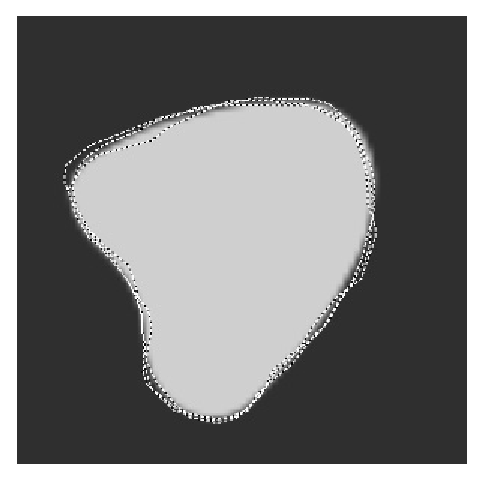
\includegraphics[height=5cm]{mcr3b.eps}
   \end{tabular}
   \end{center}
   \caption[example] 
%>>>> use \label inside caption to get Fig. number with \ref{}
   { \label{fig:example} 
Figure captions are used to describe the figure and help the reader understand it's significance.  The caption should be centered underneath the figure and set in 9-point font.  It is preferable for figures and tables to be placed at the top or bottom of the page. LaTeX tends to adhere to this standard.}
   \end{figure} 

\section{MULTIMEDIA FIGURES - VIDEO AND AUDIO FILES}

Video and audio files can be included for publication. See Tab.~\ref{tab:Multimedia-Specifications} for the specifications for the mulitimedia files. Use a screenshot or another .jpg illustration for placement in the text. Use the file name to begin the caption. The text of the caption must end with the text ``http://dx.doi.org/doi.number.goes.here'' which tells the SPIE editor where to insert the hyperlink in the digital version of the manuscript. 

Here is a sample illustration and caption for a multimedia file:

   \begin{figure} [ht]
   \begin{center}
   \begin{tabular}{c} 
   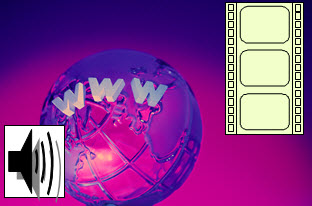
\includegraphics[height=5cm]{MultimediaFigure.jpg}
	\end{tabular}
	\end{center}
   \caption[example] 
   { \label{fig:video-example} 
A label of “Video/Audio 1, 2, …” should appear at the beginning of the caption to indicate to which multimedia file it is linked . Include this text at the end of the caption: \url{http://dx.doi.org/doi.number.goes.here}}
   \end{figure} 
   
   \begin{table}[ht]
\caption{Information on video and audio files that must accompany a manuscript submission.} 
\label{tab:Multimedia-Specifications}
\begin{center}       
\begin{tabular}{|l|l|l|}
\hline
\rule[-1ex]{0pt}{3.5ex}  Item & Video & Audio  \\
\hline
\rule[-1ex]{0pt}{3.5ex}  File name & Video1, video2... & Audio1, audio2...   \\
\hline
\rule[-1ex]{0pt}{3.5ex}  Number of files & 0-10 & 0-10  \\
\hline
\rule[-1ex]{0pt}{3.5ex}  Size of each file & 5 MB & 5 MB  \\
\hline
\rule[-1ex]{0pt}{3.5ex}  File types accepted & .mpeg, .mov (Quicktime), .wmv (Windows Media Player) & .wav, .mp3  \\
\hline 
\end{tabular}
\end{center}
\end{table}

\appendix    %>>>> this command starts appendixes

\section{MISCELLANEOUS FORMATTING DETAILS}
\label{sec:misc}

It is often useful to refer back (or forward) to other sections in the article.  Such references are made by section number.  When a section reference starts a sentence, Section is spelled out; otherwise use its abbreviation, for example, ``In Sec.~2 we showed...'' or ``Section~2.1 contained a description...''.  References to figures, tables, and theorems are handled the same way.

\subsection{Formatting Equations}
Equations may appear in line with the text, if they are simple, short, and not of major importance; e.g., $\beta = b/r$.  Important equations appear on their own line.  Such equations are centered.  For example, ``The expression for the field of view is
\begin{equation}
\label{eq:fov}
2 a = \frac{(b + 1)}{3c} \, ,
\end{equation}
where $a$ is the ...'' Principal equations are numbered, with the equation number placed within parentheses and right justified.  

Equations are considered to be part of a sentence and should be punctuated accordingly. In the above example, a comma follows the equation because the next line is a subordinate clause.  If the equation ends the sentence, a period should follow the equation.  The line following an equation should not be indented unless it is meant to start a new paragraph.  Indentation after an equation is avoided in LaTeX by not leaving a blank line between the equation and the subsequent text.

References to equations include the equation number in parentheses, for example, ``Equation~(\ref{eq:fov}) shows ...'' or ``Combining Eqs.~(2) and (3), we obtain...''  Using a tilde in the LaTeX source file between two characters avoids unwanted line breaks.

\subsection{Formatting Theorems}

To include theorems in a formal way, the theorem identification should appear in a 10-point, bold font, left justified and followed by a period.  The text of the theorem continues on the same line in normal, 10-point font.  For example, 

\noindent\textbf{Theorem 1.} For any unbiased estimator...

Formal statements of lemmas and algorithms receive a similar treatment.

\end{comment}


\acknowledgments % equivalent to \section*{ACKNOWLEDGMENTS}       
 
This unnumbered section is used to identify those who have aided the authors in understanding or accomplishing the work presented and to acknowledge sources of funding.  

% References
\bibliography{report} % bibliography data in report.bib
\bibliographystyle{spiebib} % makes bibtex use spiebib.bst

\end{document} 
